\documentclass[11pt]{article}

\usepackage{latexsym}
\usepackage{amsmath}
\usepackage{amssymb}
\usepackage{amsthm}
\usepackage{graphicx}
\usepackage{wrapfig}
\usepackage{pseudocode}
\usepackage{url}
\usepackage[backref, colorlinks=true, citecolor=red, urlcolor=blue, pdfauthor={Jyh-Ming Lien}]{hyperref}
\usepackage{subfigure}
\usepackage{enumitem}

\newcommand{\handout}[5]{
  \noindent
  \begin{center}
  \framebox{
    \vbox{
      \hbox to 5.78in { {\bf } \hfill #2 }
      \vspace{4mm}
      \hbox to 5.78in { {\Large \hfill #5  \hfill} }
      \vspace{2mm}
      \hbox to 5.78in { {\em #3 \hfill #4} }
    }
  }
  \end{center}
  \vspace*{4mm}
}

\newcommand{\lecture}[4]{\handout{#1}{#2}{#3}{}{Report for #1}}

\newtheorem{theorem}{Theorem}
\newtheorem{corollary}[theorem]{Corollary}
\newtheorem{lemma}[theorem]{Lemma}
\newtheorem{observation}[theorem]{Observation}
\newtheorem{proposition}[theorem]{Proposition}
\newtheorem{definition}[theorem]{Definition}
\newtheorem{claim}[theorem]{Claim}
\newtheorem{fact}[theorem]{Fact}
\newtheorem{assumption}[theorem]{Assumption}

% 1-inch margins, from fullpage.sty by H.Partl, Version 2, Dec. 15, 1988.
\topmargin 0pt
\advance \topmargin by -\headheight
\advance \topmargin by -\headsep
\textheight 8.9in
\oddsidemargin 0pt
\evensidemargin \oddsidemargin
\marginparwidth 0.5in
\textwidth 6.5in

\parindent 0in
\parskip 1.5ex
%\renewcommand{\baselinestretch}{1.25}

\begin{document}

\lecture{Advance Algorithm Programming Assignment 1 }{Fall 2015}{Yeojin Kim}{---}


\section{Implementation Details}
\subsection{Algorithm}\label{algorithm}
The crust algorithm is as follows:
\setenumerate[2]{label=\alph*.}
\begin{enumerate}
\item Compute Voronoi diagram of the given points.
\begin{enumerate}
\item Create points in 4D using 3 coordinates : $\mathbf{(x,y, z, x^2+y^2+z^2)}$
\item Compute convex hull in 4D by calling qhull\cite{Qhull} with 4D points.
\item Loop through all facets in 4D convex hull,
\begin{enumerate}
\item If this facet is in lower hull and the volume of facet is not zero, 
\item Compute the center of facet. This is a Voronoi vertex of the vertices (i.e. Voronoi cites) in facet.
\item Save the Voronoi vertex and bounded/unbounded information in each vertex in facet. 
\end{enumerate}
\end{enumerate}
\item Find a pole and an antipole. Loop through all Voronoi cites,
\begin{enumerate}
\item If Voronoi cell is unbounded, find an average normal $n^{+}$ of adjacent triangles.
\item  If Voronoi cell is bounded, find a pole comparing the distance between the cite $c$ and Voronoi vertices. The farthest Voronoi vertex becomes pole $p$. Compute a normal vector $n^{+}$ from vector $\overrightarrow{cp}$.
\item Compute an antipole using normal $n^{+}$. Voronoi vertex which has the smallest value from inner product with $n^{+}$ is an antipole.
\end{enumerate}
\item Apply Delaunay triangulation to the union set of sample points, poles, and antipoles. Print faces only when the face consists of sample points. 
\end{enumerate}

\subsection{Software}
OS : Window 8.1K\\
IDE : Visual Studio 2013\\

\section{Example Output} \label{Example}
At the first time, I removed some points which have the distance between the cite and vertex is bigger than 10000, but in some cases I cannot obtain fair crust of models. 
Therefore, I set the distance threshold as 1000 for all models. In Fig. \ref{fig:cube} - Fig. \ref{fig:teeth}, (a) shows the result of crust. (b) - (c) shows the inside/outside of sample points. Red points are given sample points and green points are poles and antipoles. Through (b) - (c), we can observe that poles and antipoles lie close to the medial axis. 

\section{Know bugs/limitations}
First, I set some thresholds for fair results. In section \ref{algorithm}, I skipped Voronoi centers in tetrahedron which has very small volume, which is close to zero. Even if I used the DELAUNAY options, the computing Voronoi vertices generates points which are almost coplanar with four vertices and it makes unexpected holes. So I give the condition about volume. Also I mentioned in Section \ref{Example}, I removed some points far away from the cites. I set this value manually regardless of models. \\
In addition, if program loops through vertices not facets, it can compute crust more fast. It can compute a Voronoi vertex, a pole and an antipole at the same time, while visiting a cite once. 
\bibliographystyle{plain}
\bibliography{report}
\begin{figure*}[hbt]
 \centering
  \subfigure[]{
    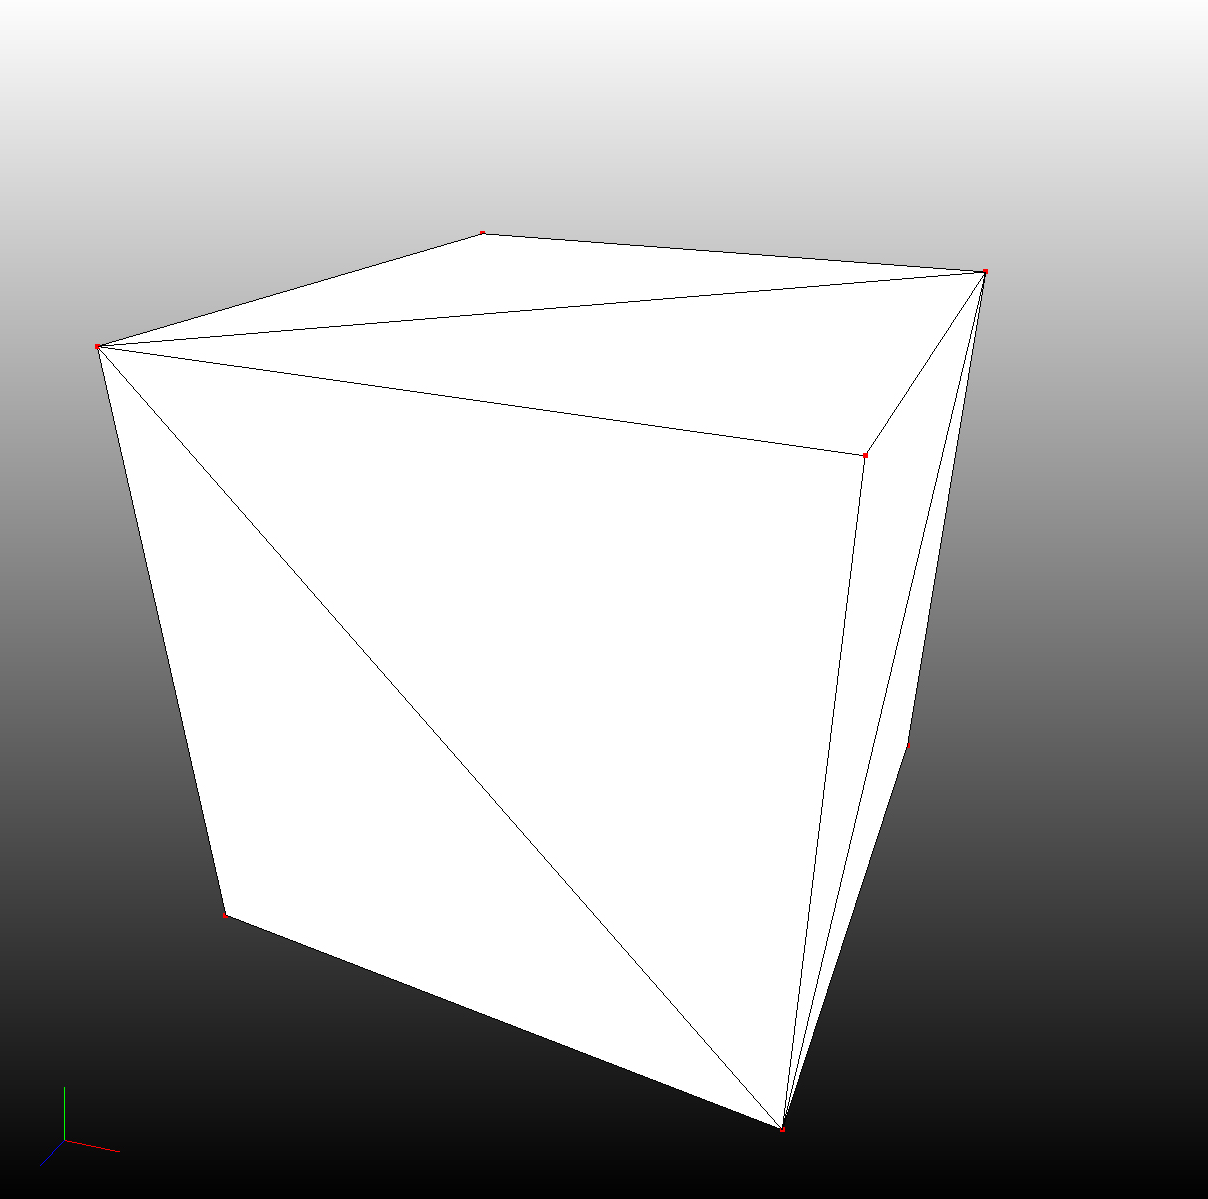
\includegraphics[width=0.42\textwidth]{img/cube01.png}
    \label{fig:cube1}
  }\hspace{-3mm}
  \subfigure[]{
     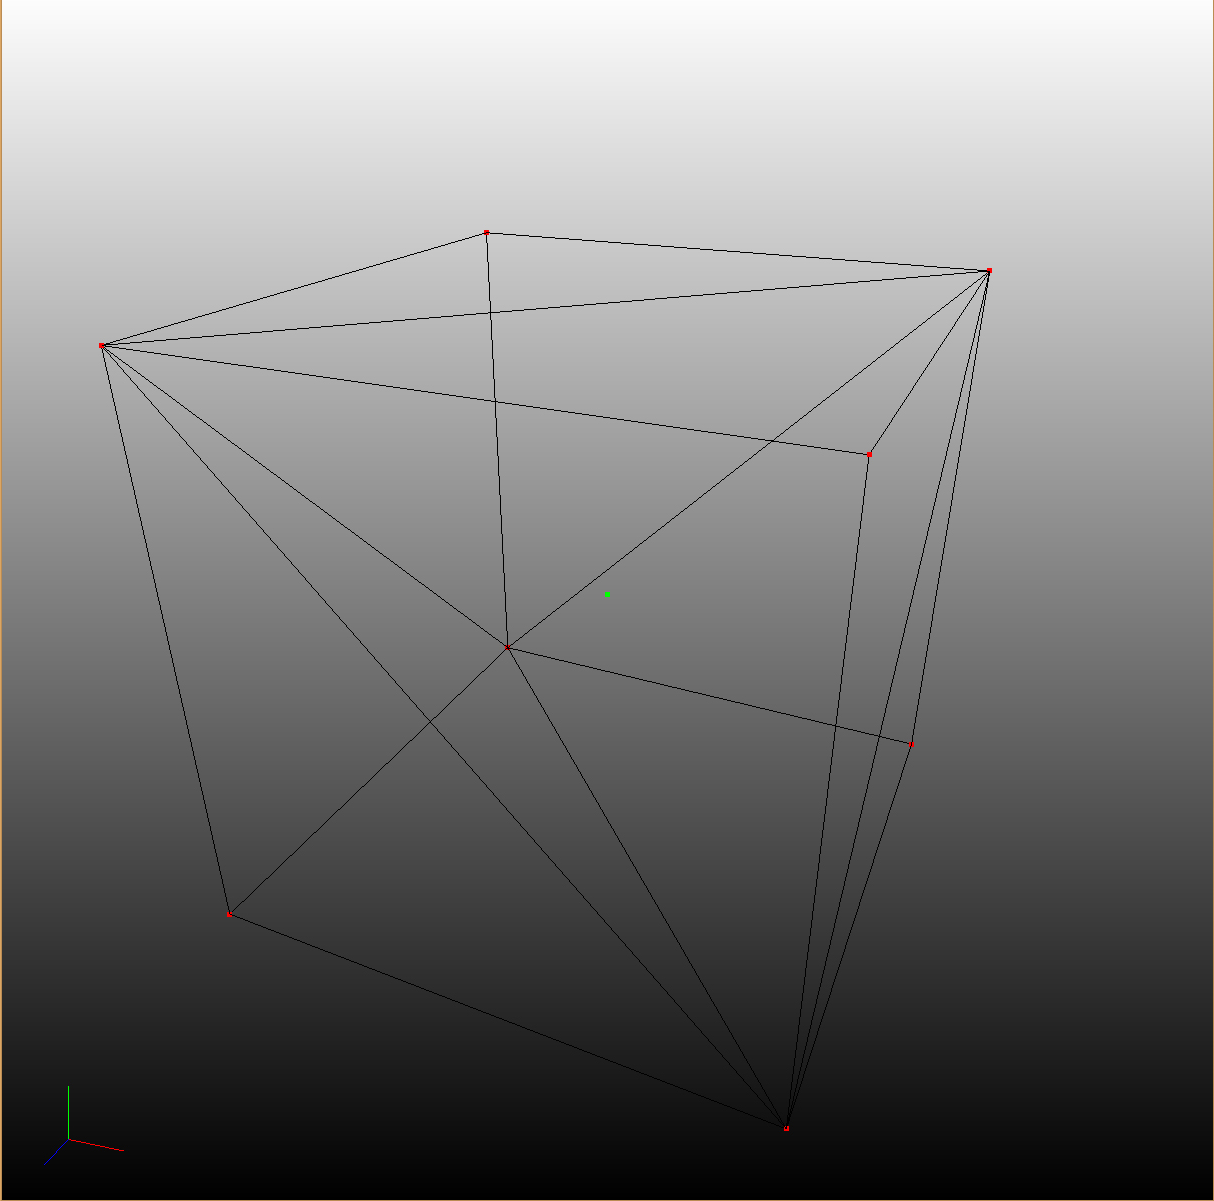
\includegraphics[width=0.42\textwidth]{img/cube02.png}
     \label{fig:cube2}
  }\hspace{-3mm}
    \caption{A cube example\label{fig:cube}}
\end{figure*}
\begin{figure*}[hbt]
 \centering
  \subfigure[]{
    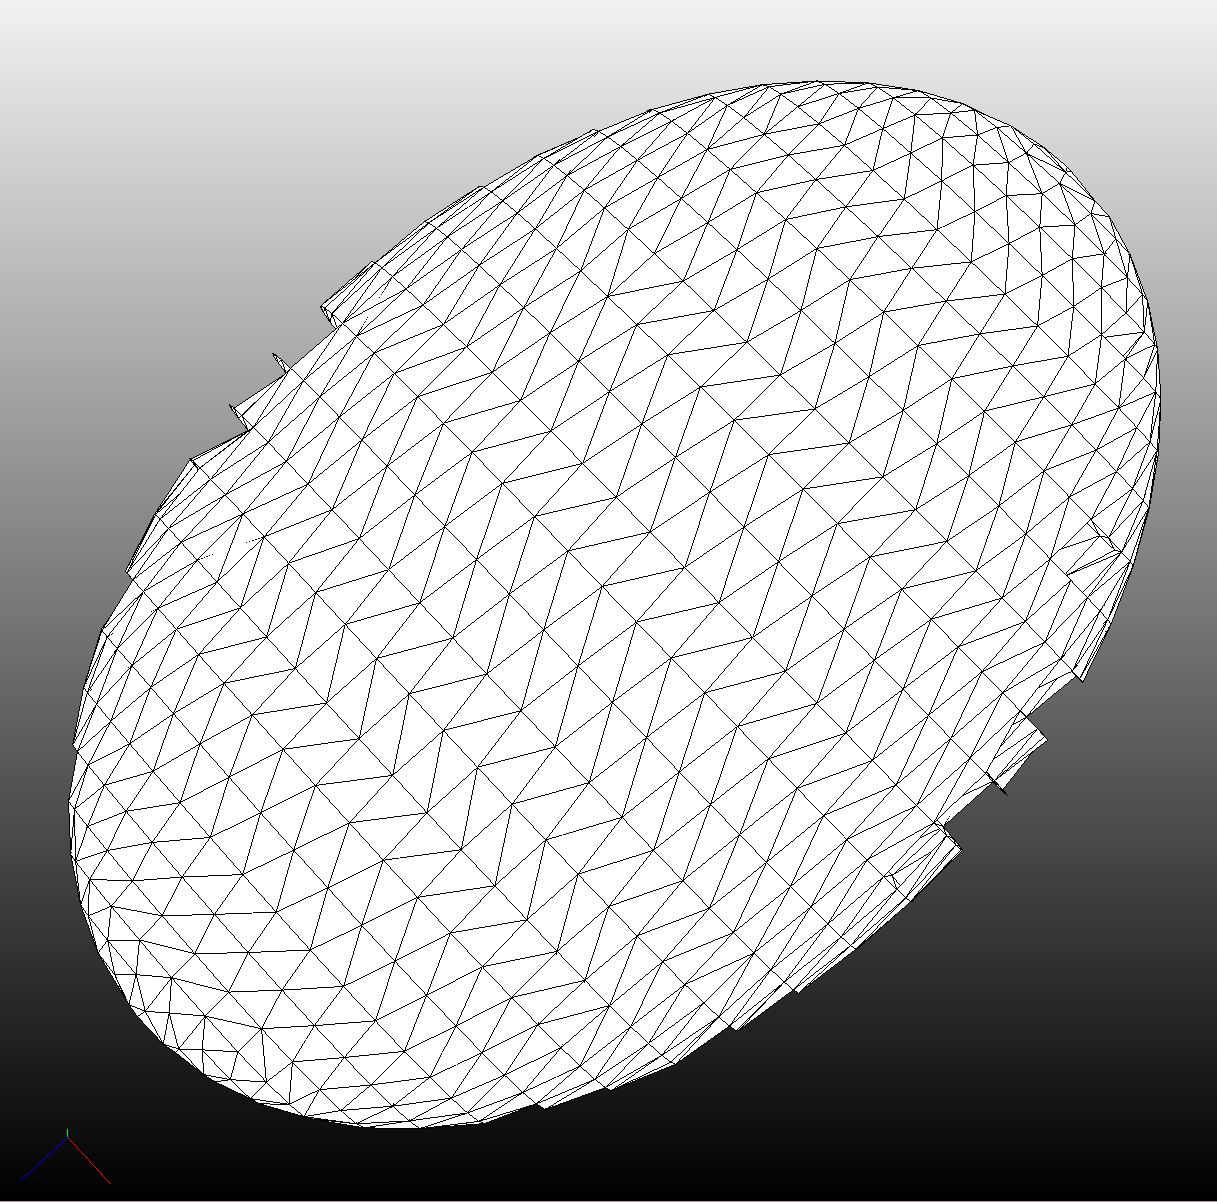
\includegraphics[width=0.32\textwidth]{img/ellipsoid01.png}
    \label{fig:ellipsoid1}
  }\hspace{-3mm}
  \subfigure[]{
     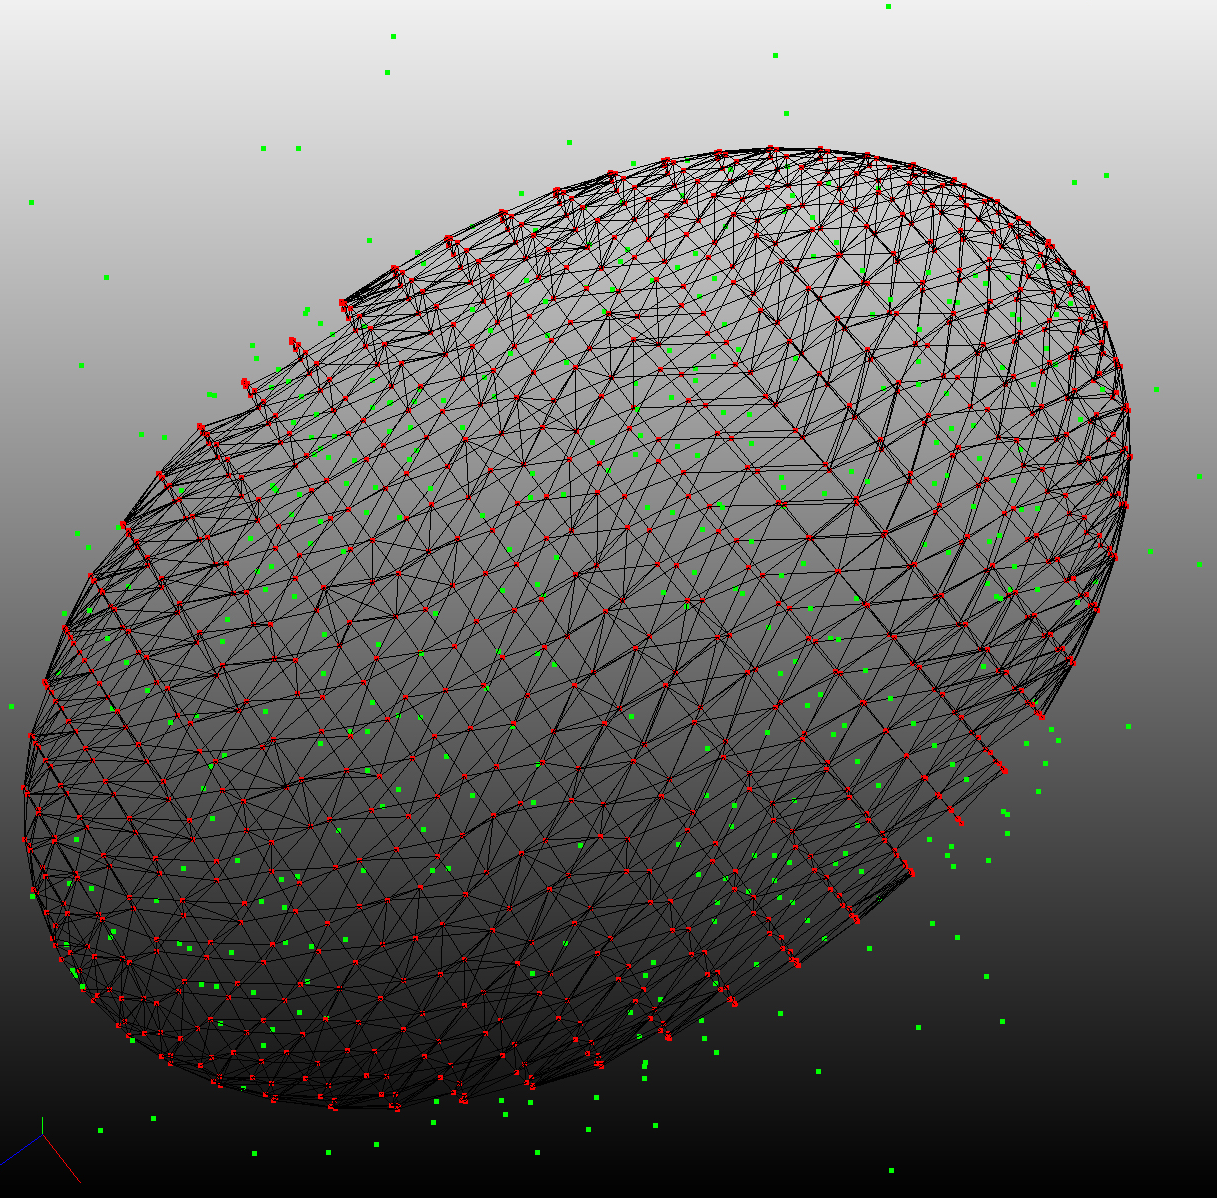
\includegraphics[width=0.32\textwidth]{img/ellipsoid02.png}
     \label{fig:ellipsoid2}
  }\hspace{-3mm}
  \subfigure[]{
    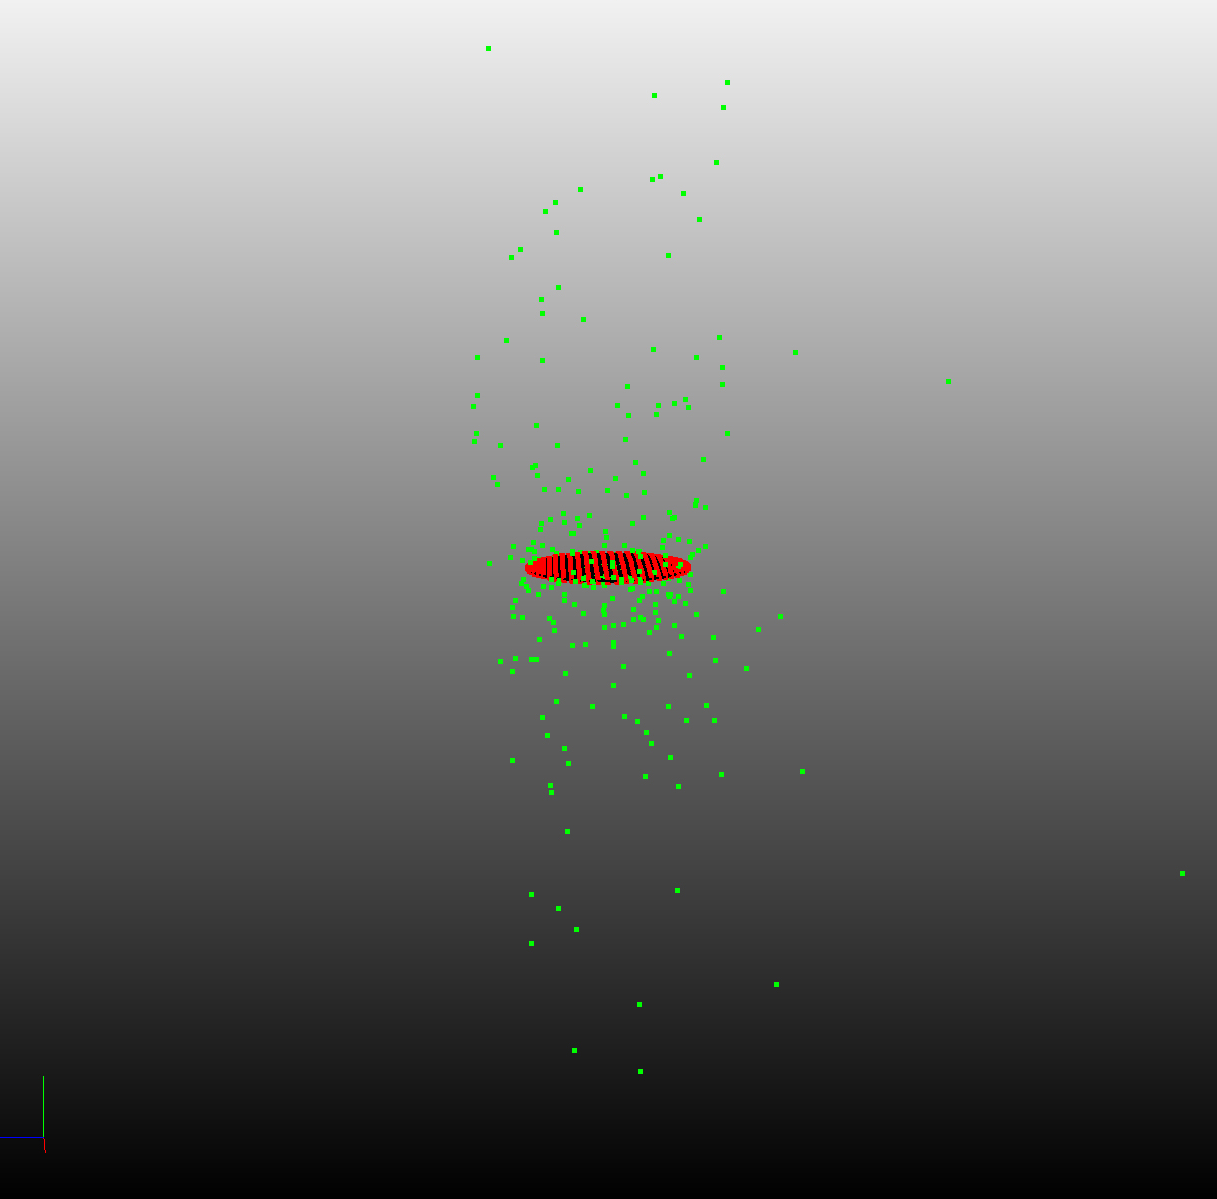
\includegraphics[width=0.32\textwidth]{img/ellipsoid03.png}
     \label{fig:ellipsoid3}
  }\hspace{-3mm}
  \caption{An ellipsoid example \label{fig:ellipsoid}}
\end{figure*}
\begin{figure*}[hbt]
 \centering
  \subfigure[]{
    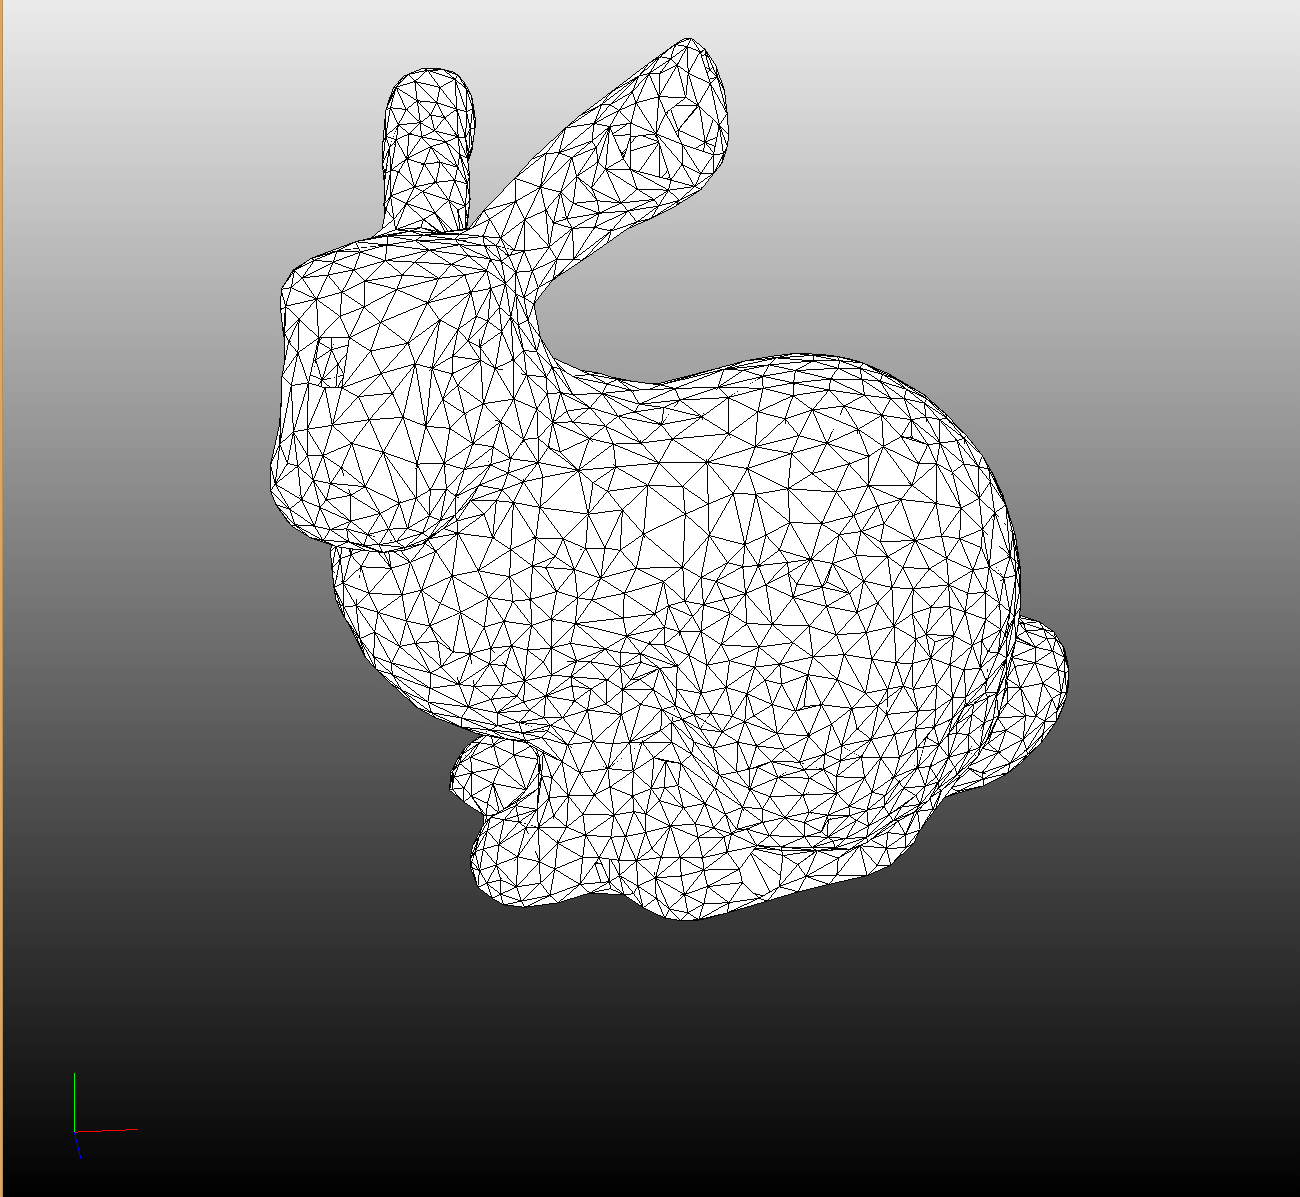
\includegraphics[width=0.32\textwidth]{img/bunny01.png}
    \label{fig:bunny1}
  }\hspace{-3mm}
  \subfigure[]{
     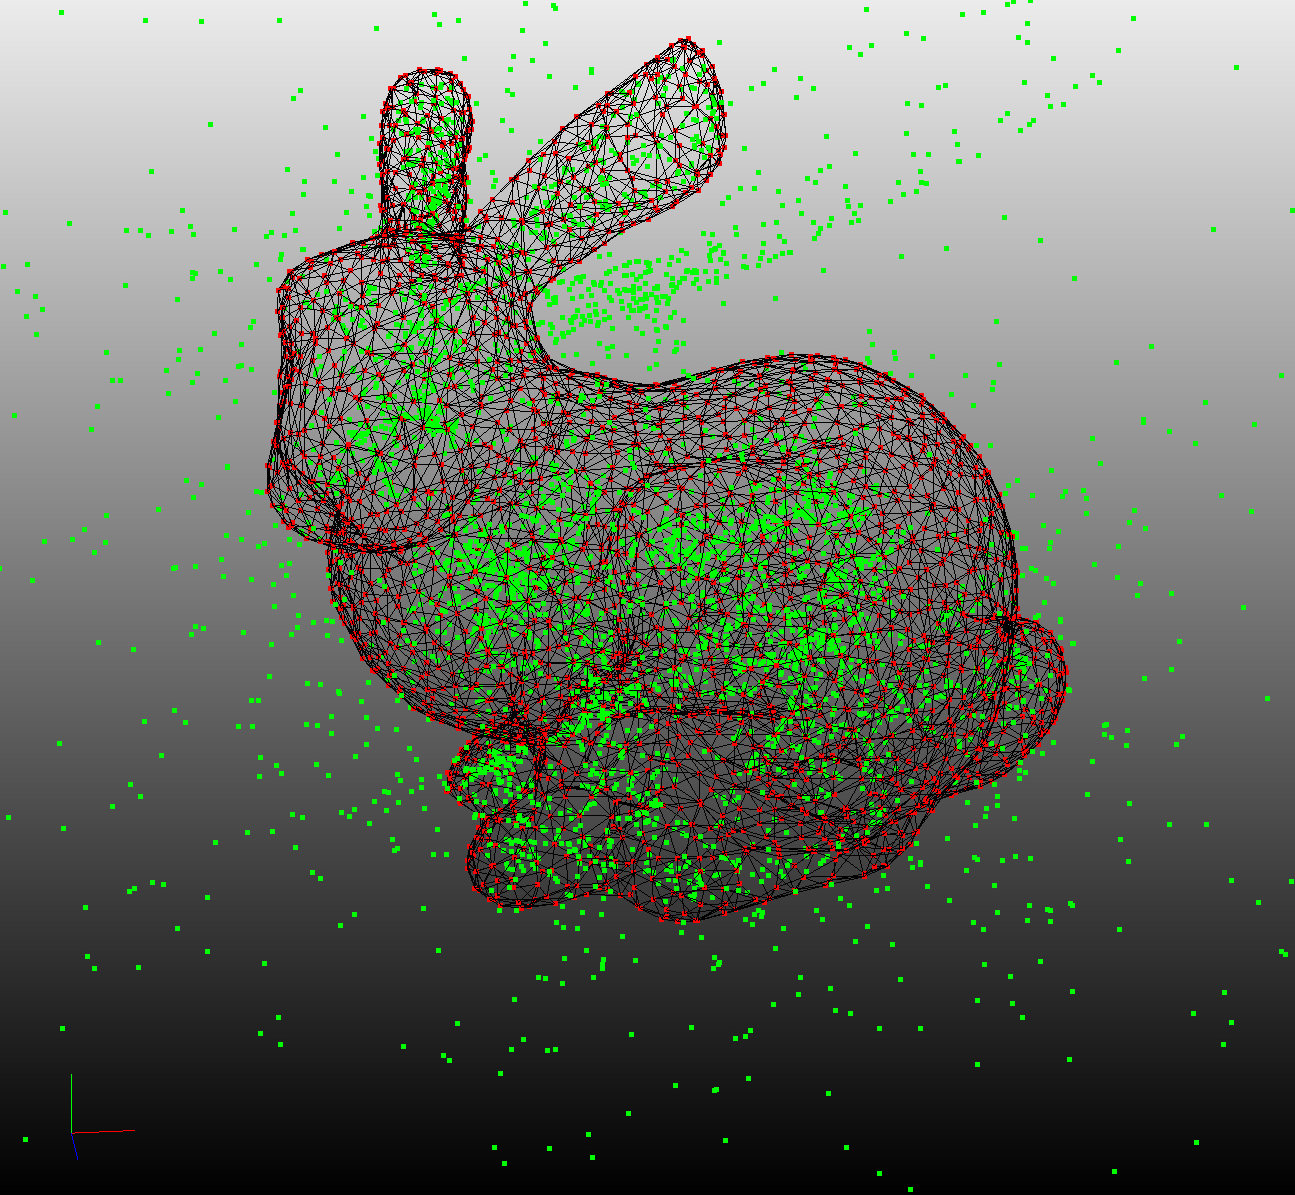
\includegraphics[width=0.32\textwidth]{img/bunny02.png}
     \label{fig:bunny2}
  }\hspace{-3mm}
  \subfigure[]{
    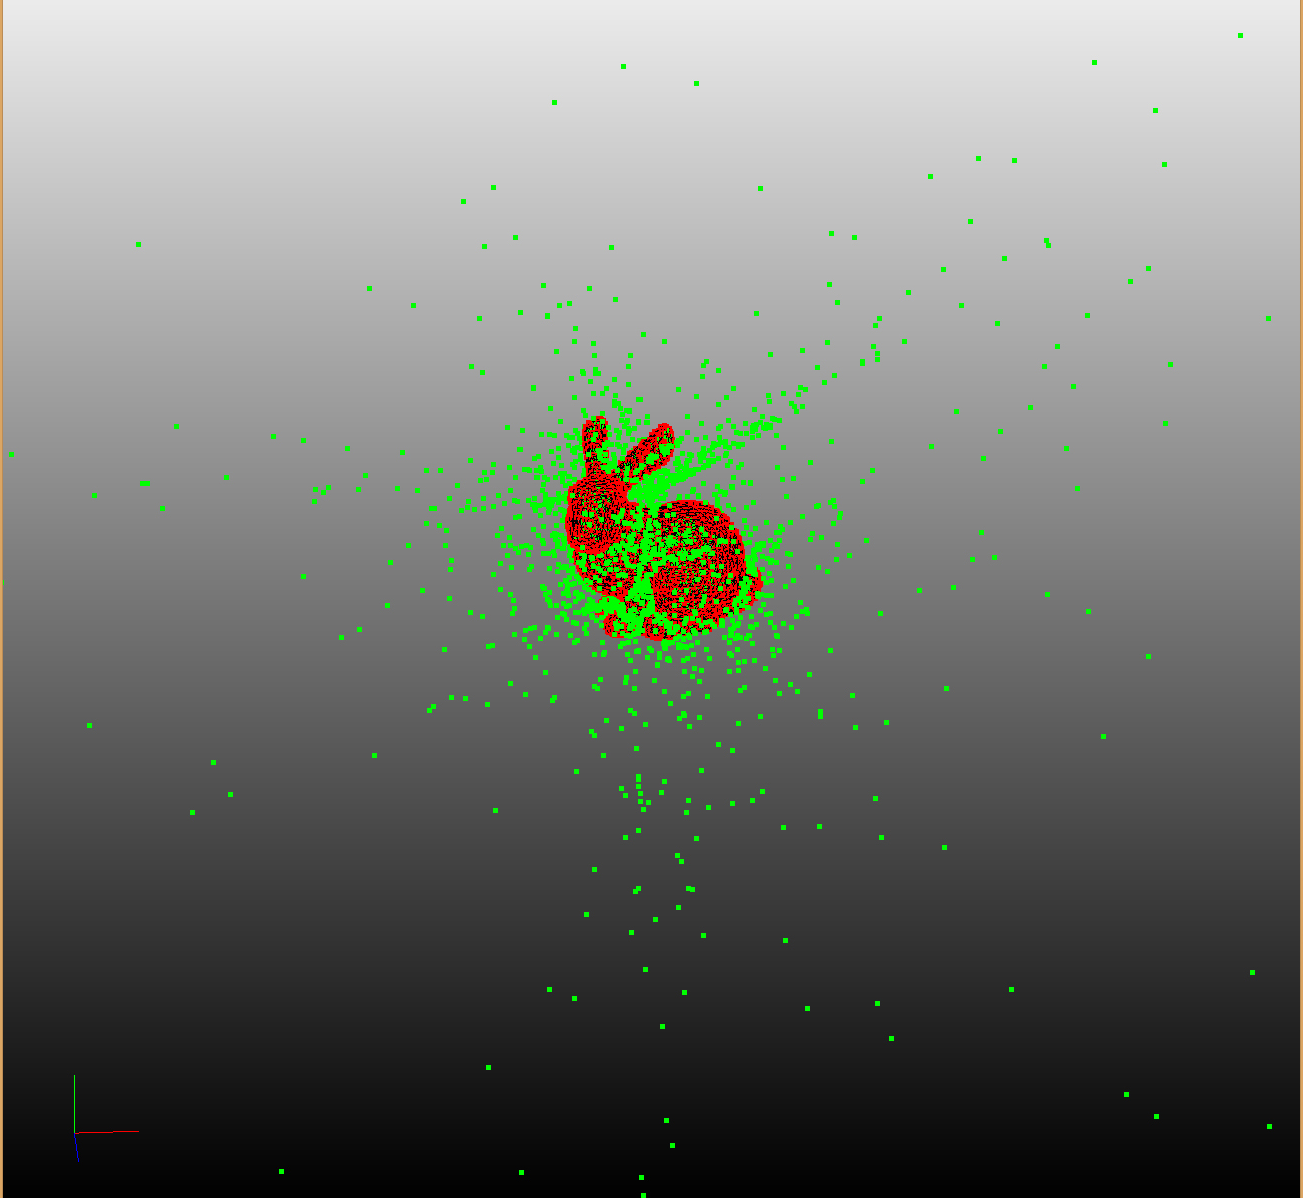
\includegraphics[width=0.32\textwidth]{img/bunny03.png}
     \label{fig:bunny3}
  }\hspace{-3mm}
  \caption{A bunny example \label{fig:bunny}}
\end{figure*}
\begin{figure*}[hbt]
 \centering
  \subfigure[]{
    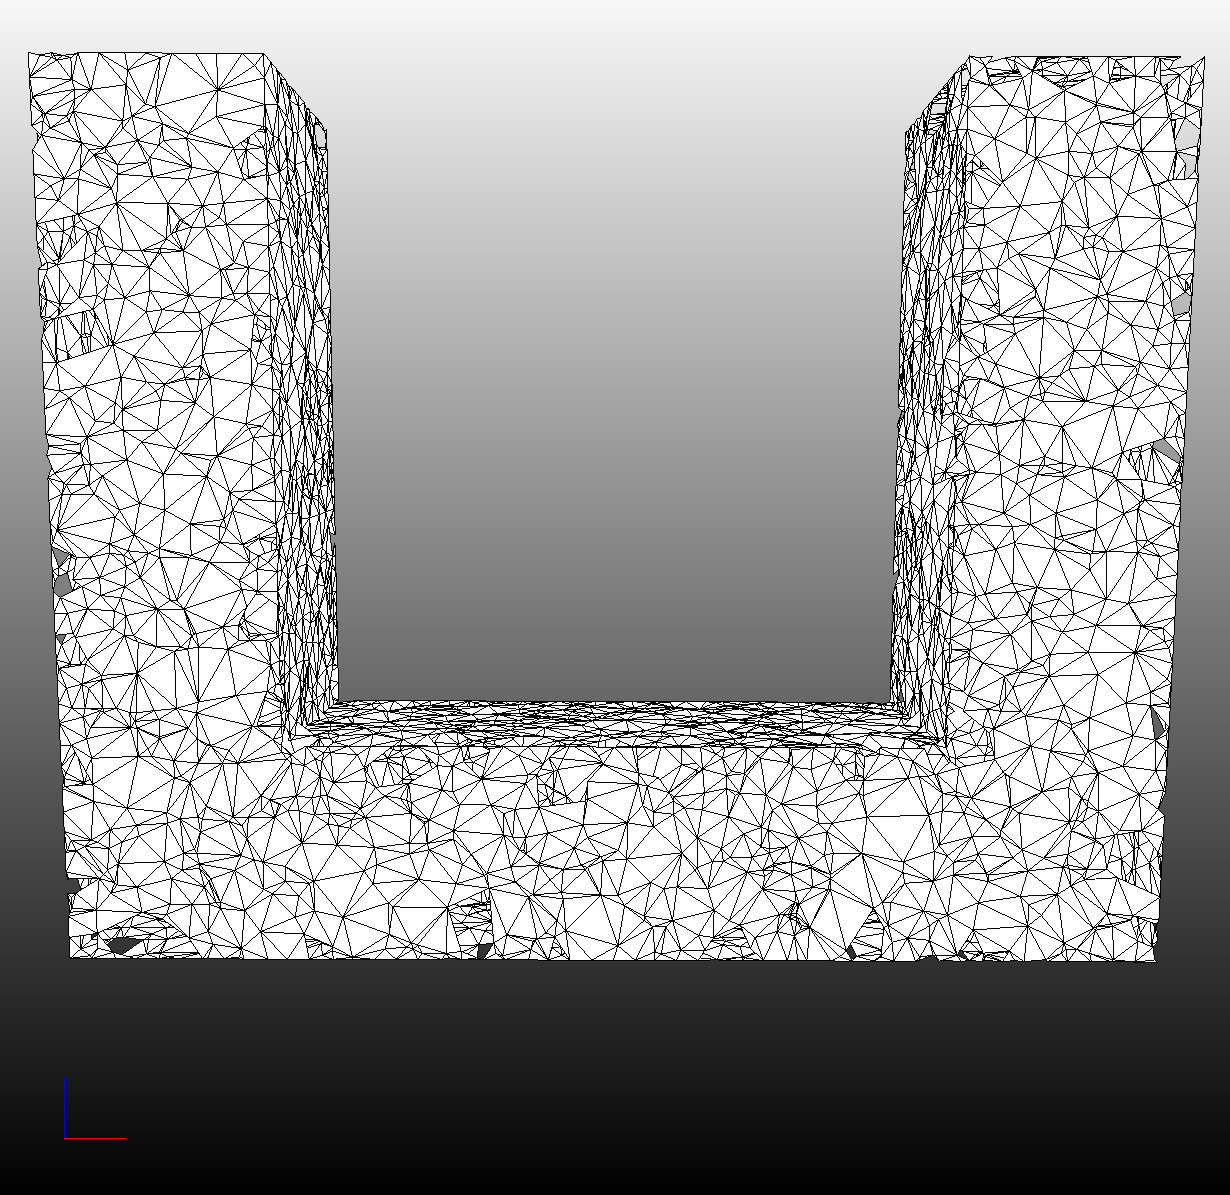
\includegraphics[width=0.32\textwidth]{img/U01.png}
    \label{fig:u1}
  }\hspace{-3mm}
  \subfigure[]{
     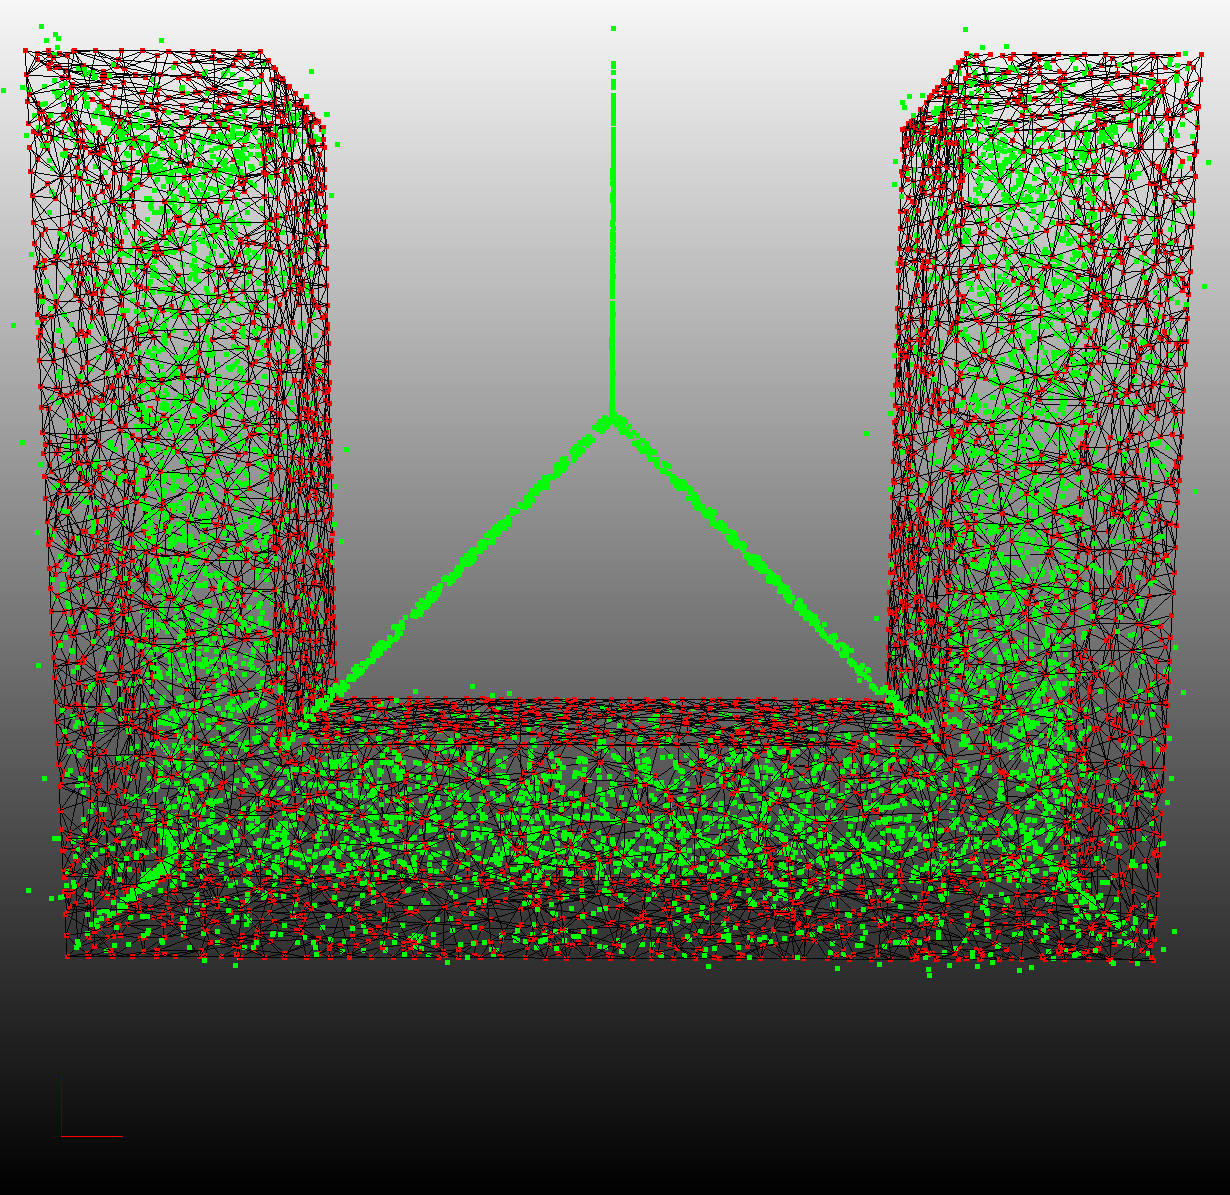
\includegraphics[width=0.32\textwidth]{img/U02.png}
     \label{fig:u2}
  }\hspace{-3mm}
  \caption{An 'U' example \label{fig:U}}
\end{figure*}
\begin{figure*}[hbt]
 \centering
  \subfigure[]{
    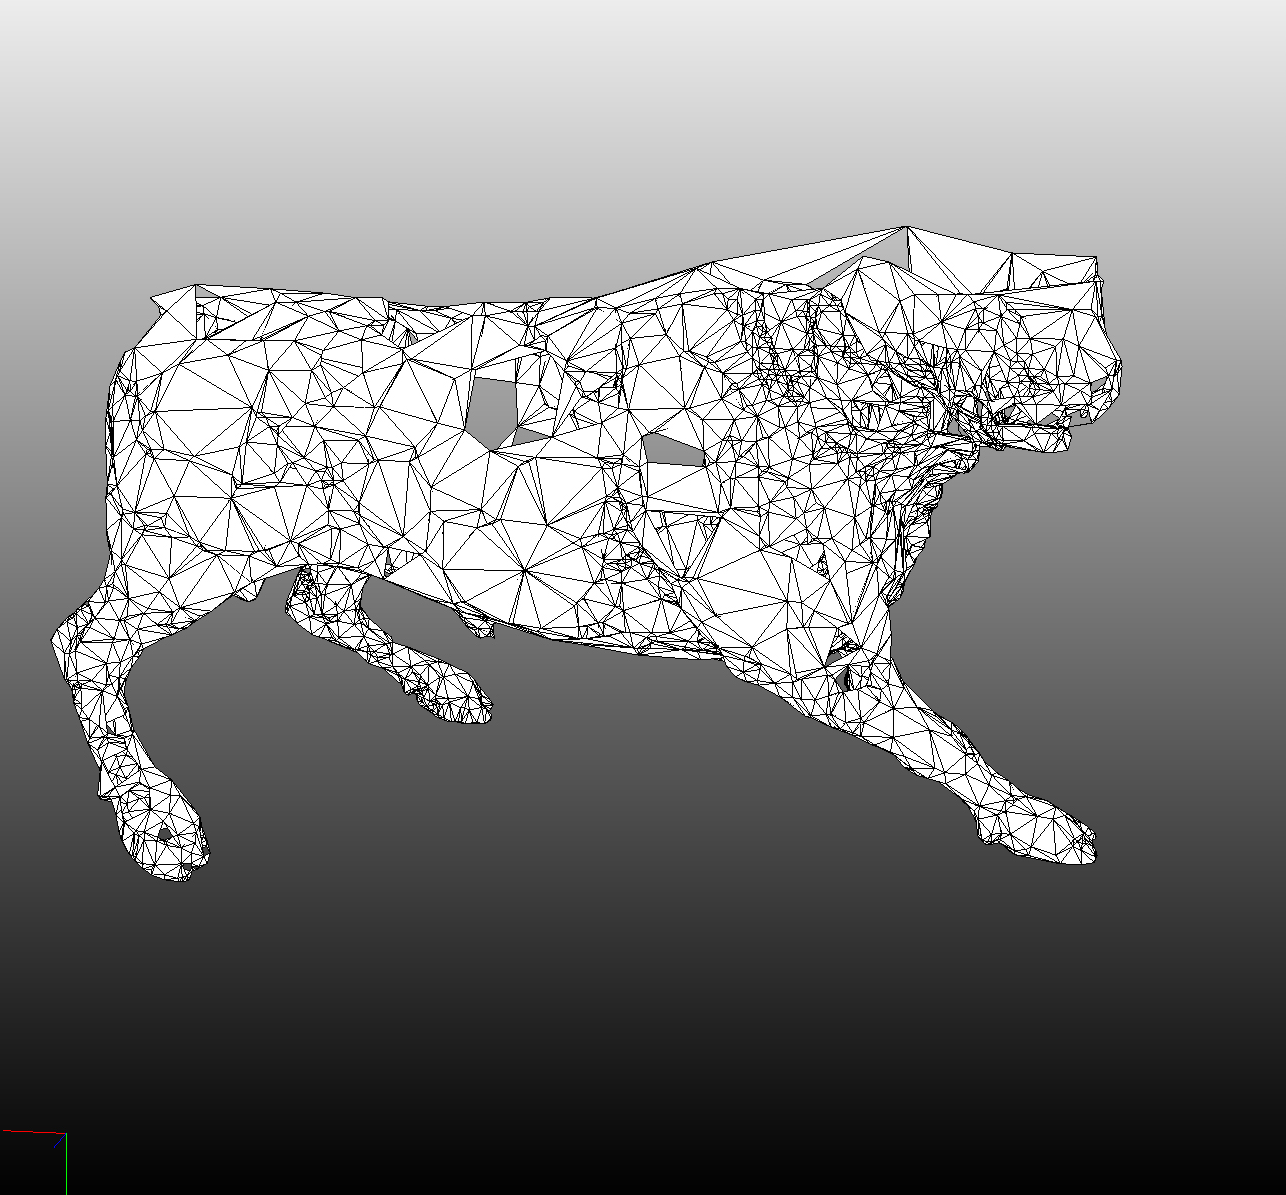
\includegraphics[width=0.32\textwidth]{img/bull01.png}
    \label{fig:bull1}
  }\hspace{-3mm}
  \subfigure[]{
     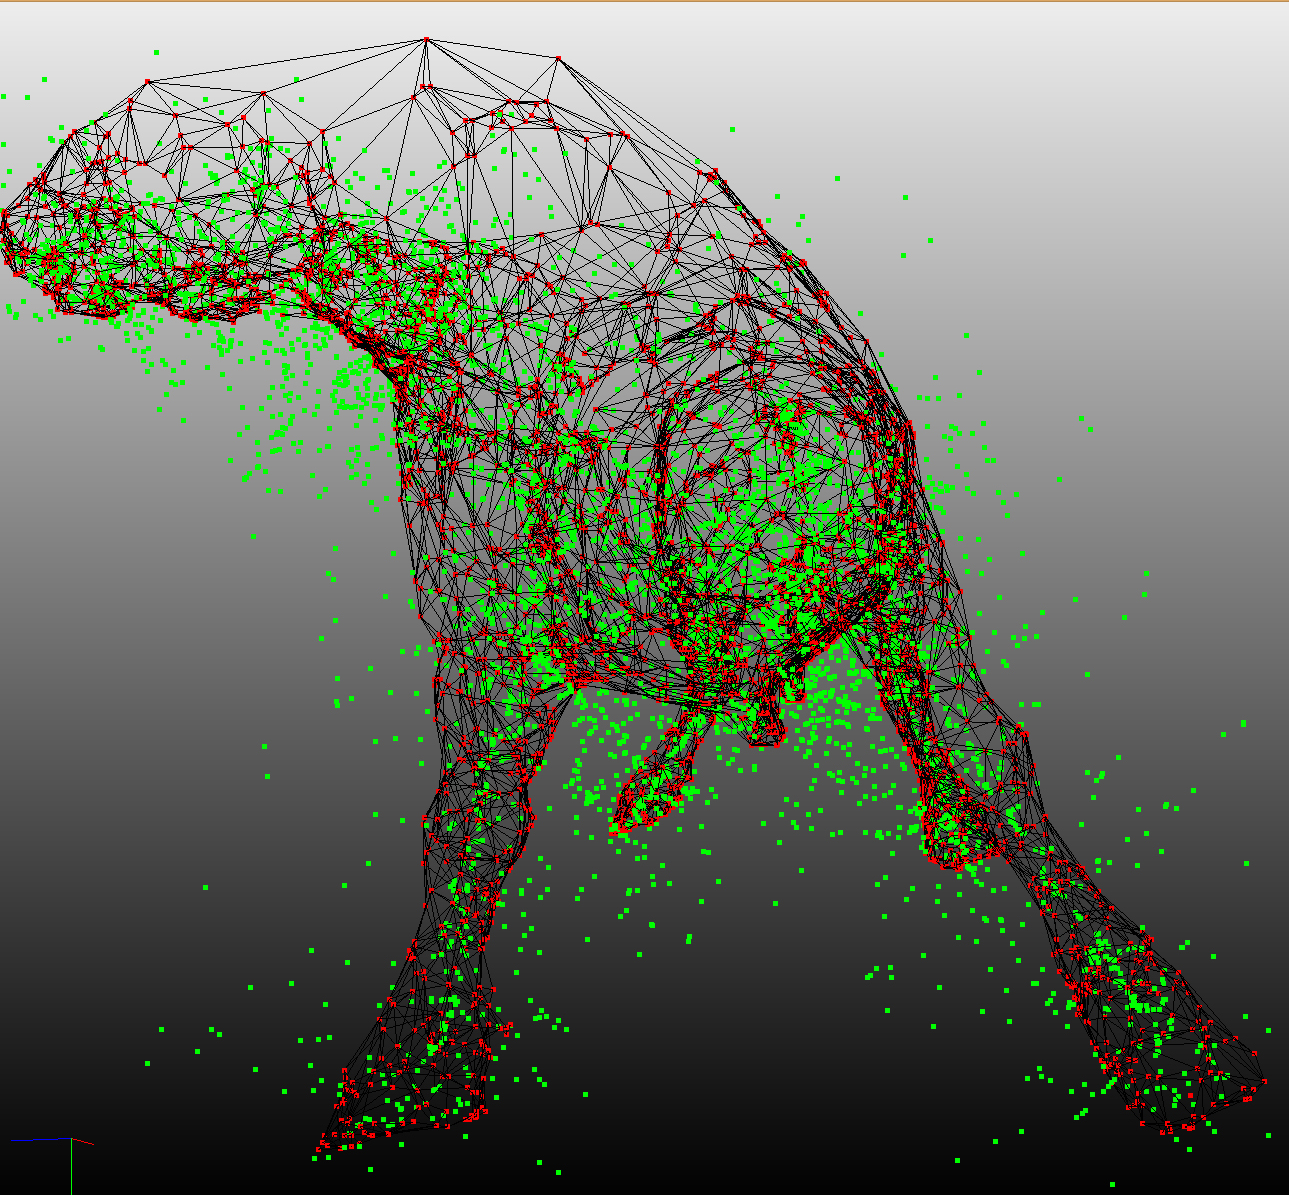
\includegraphics[width=0.32\textwidth]{img/bull02.png}
     \label{fig:bull2}
  }\hspace{-3mm}
  \subfigure[]{
    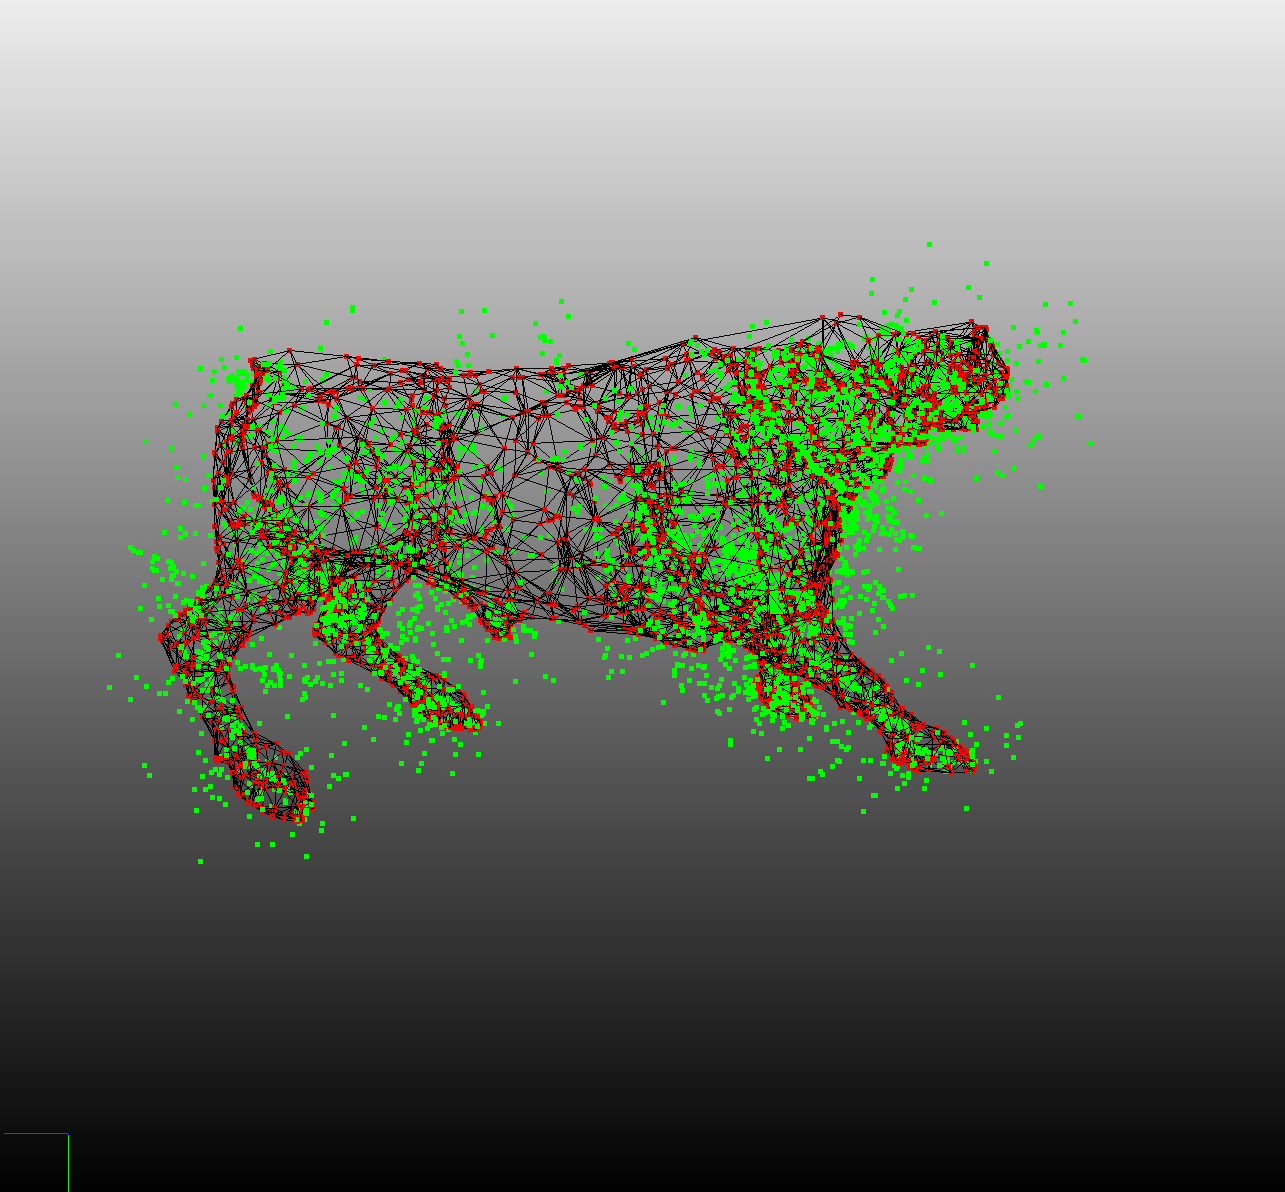
\includegraphics[width=0.32\textwidth]{img/bull03.png}
     \label{fig:bull3}
  }\hspace{-3mm}
  \caption{A bull example \label{fig:bull}}
\end{figure*}
\begin{figure*}[hbt]
 \centering
  \subfigure[]{
    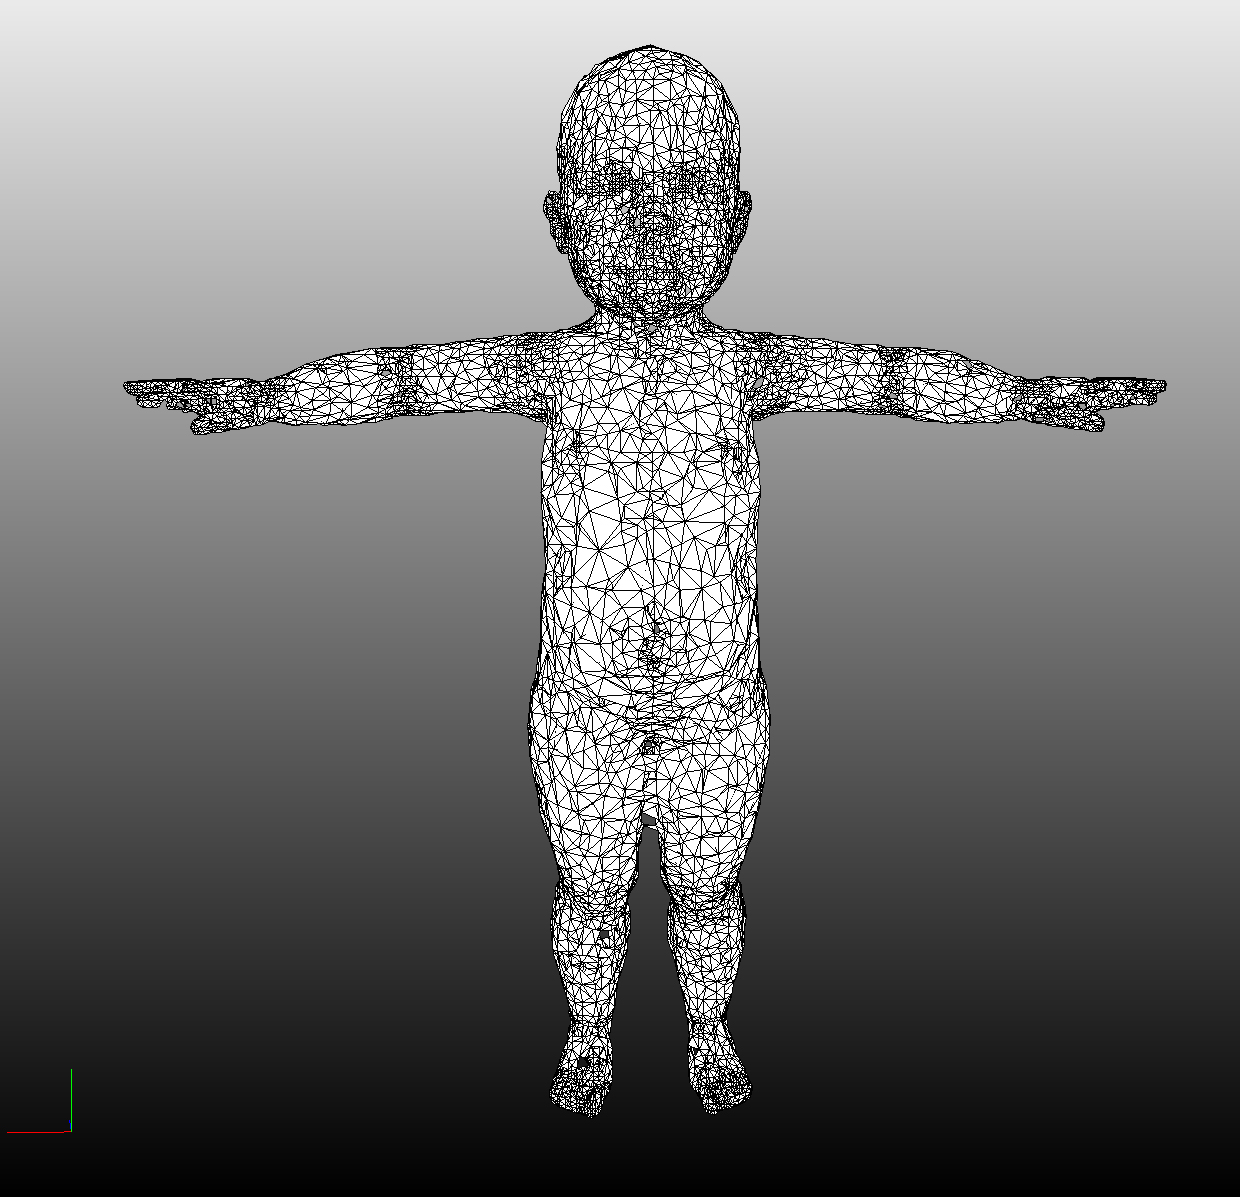
\includegraphics[width=0.32\textwidth]{img/baby01.png}
    \label{fig:bb1}
  }\hspace{-3mm}
  \subfigure[]{
     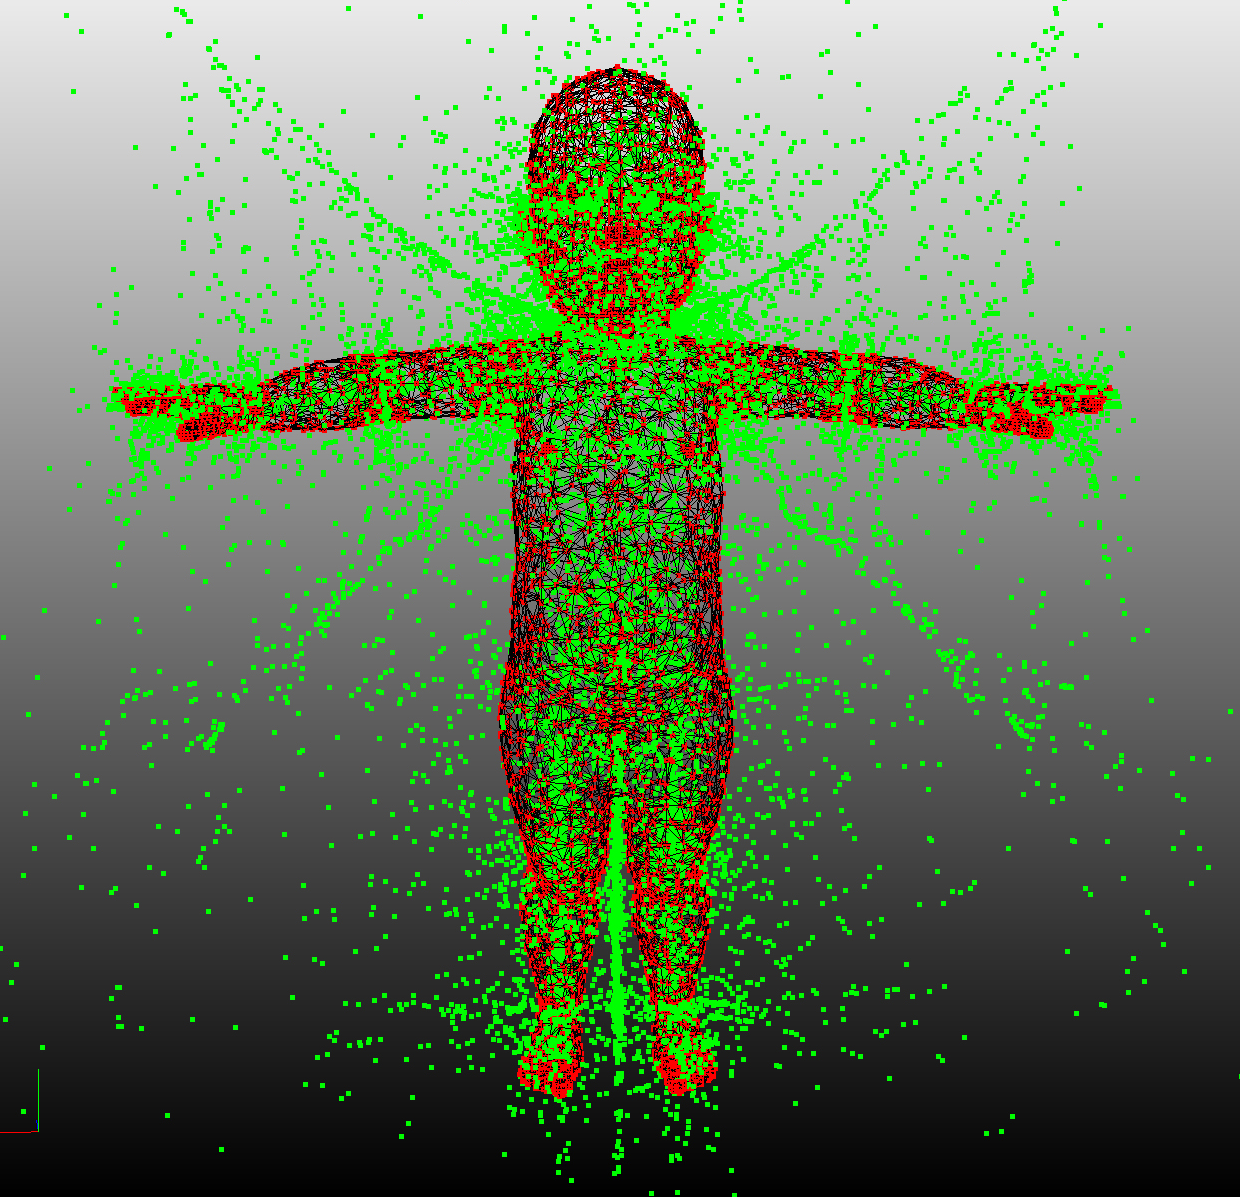
\includegraphics[width=0.32\textwidth]{img/baby02.png}
     \label{fig:bb2}
  }\hspace{-3mm}
  \subfigure[]{
    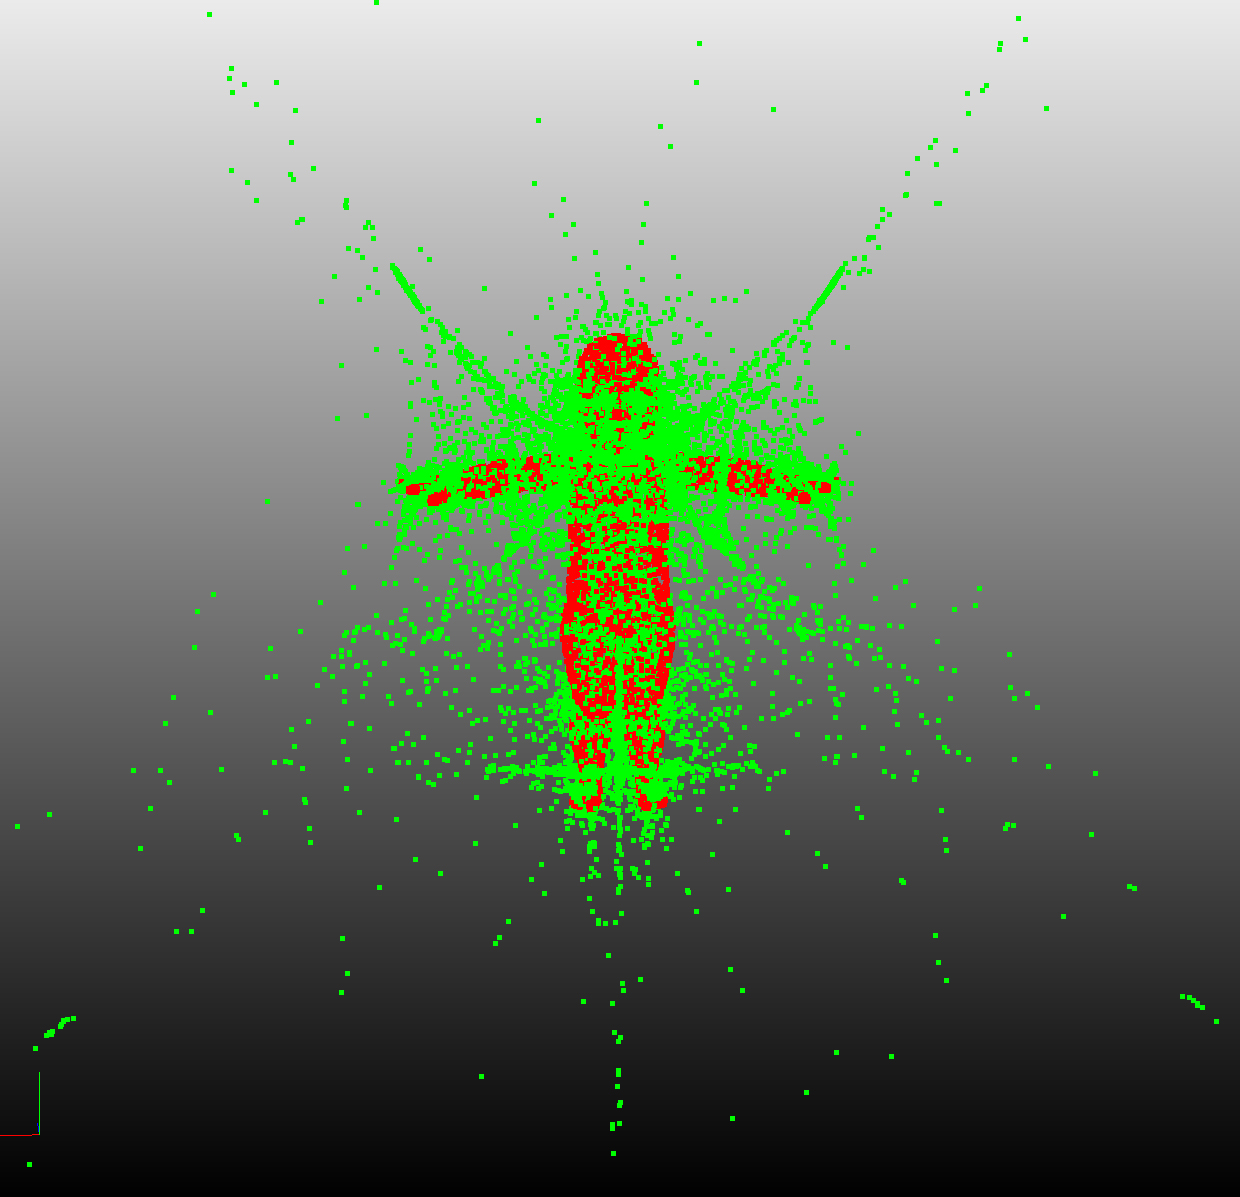
\includegraphics[width=0.32\textwidth]{img/baby03.png}
     \label{fig:bb3}
  }\hspace{-3mm}
  \caption{An baby example \label{fig:baby}}
\end{figure*}
\begin{figure*}[hbt]
 \centering
  \subfigure[]{
    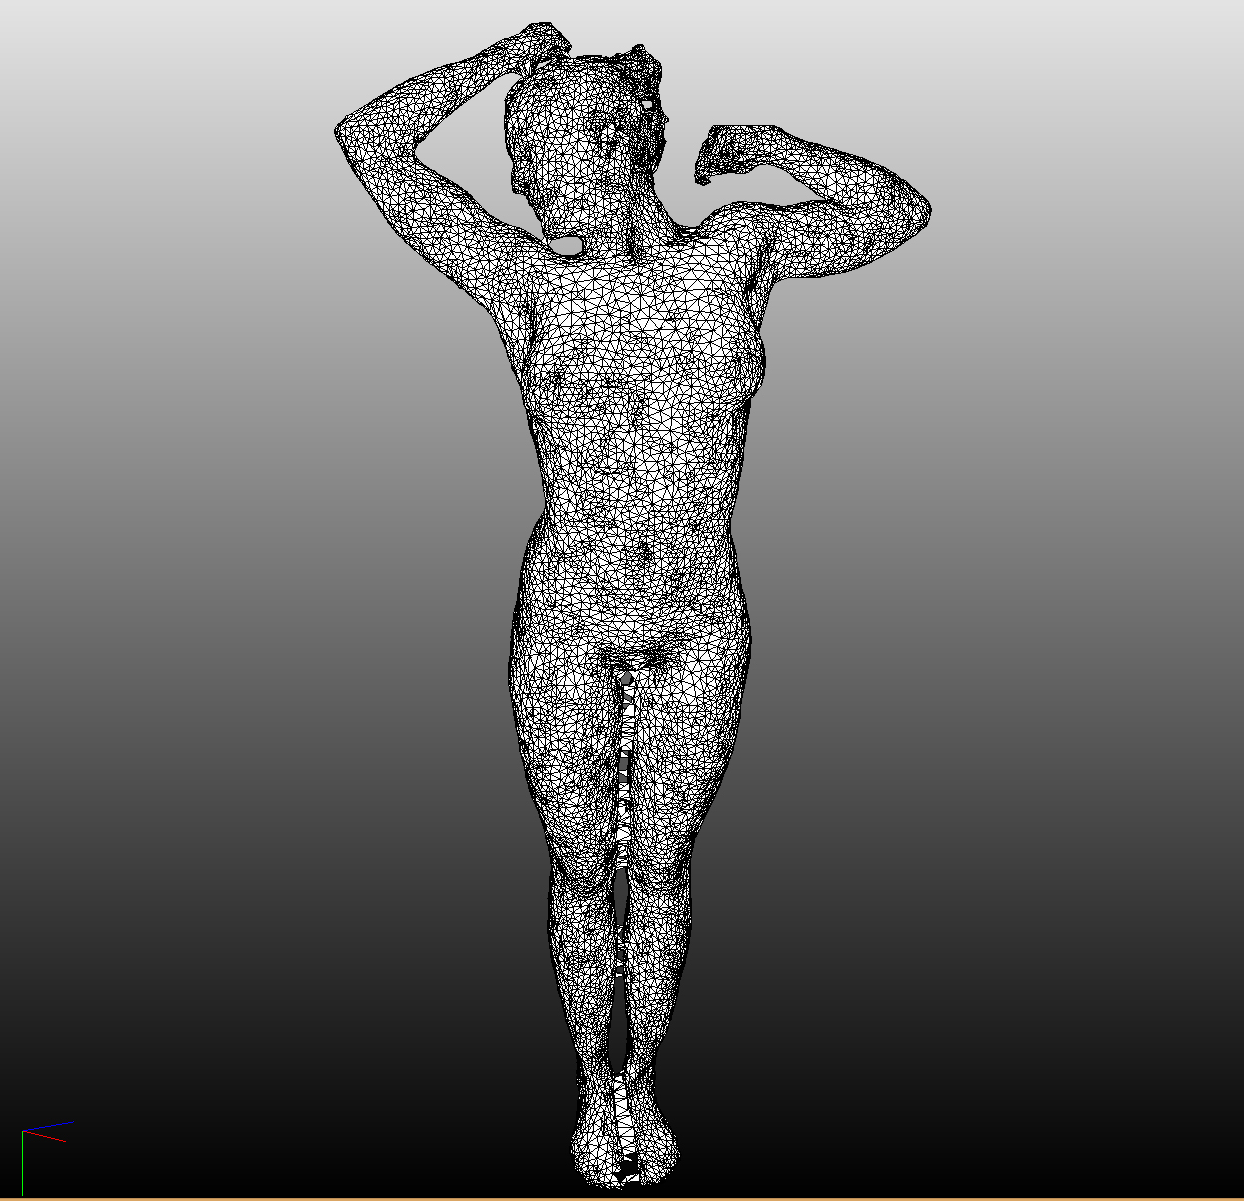
\includegraphics[width=0.32\textwidth]{img/woman01.png}
    \label{fig:woman1}
  }\hspace{-3mm}
  \subfigure[]{
     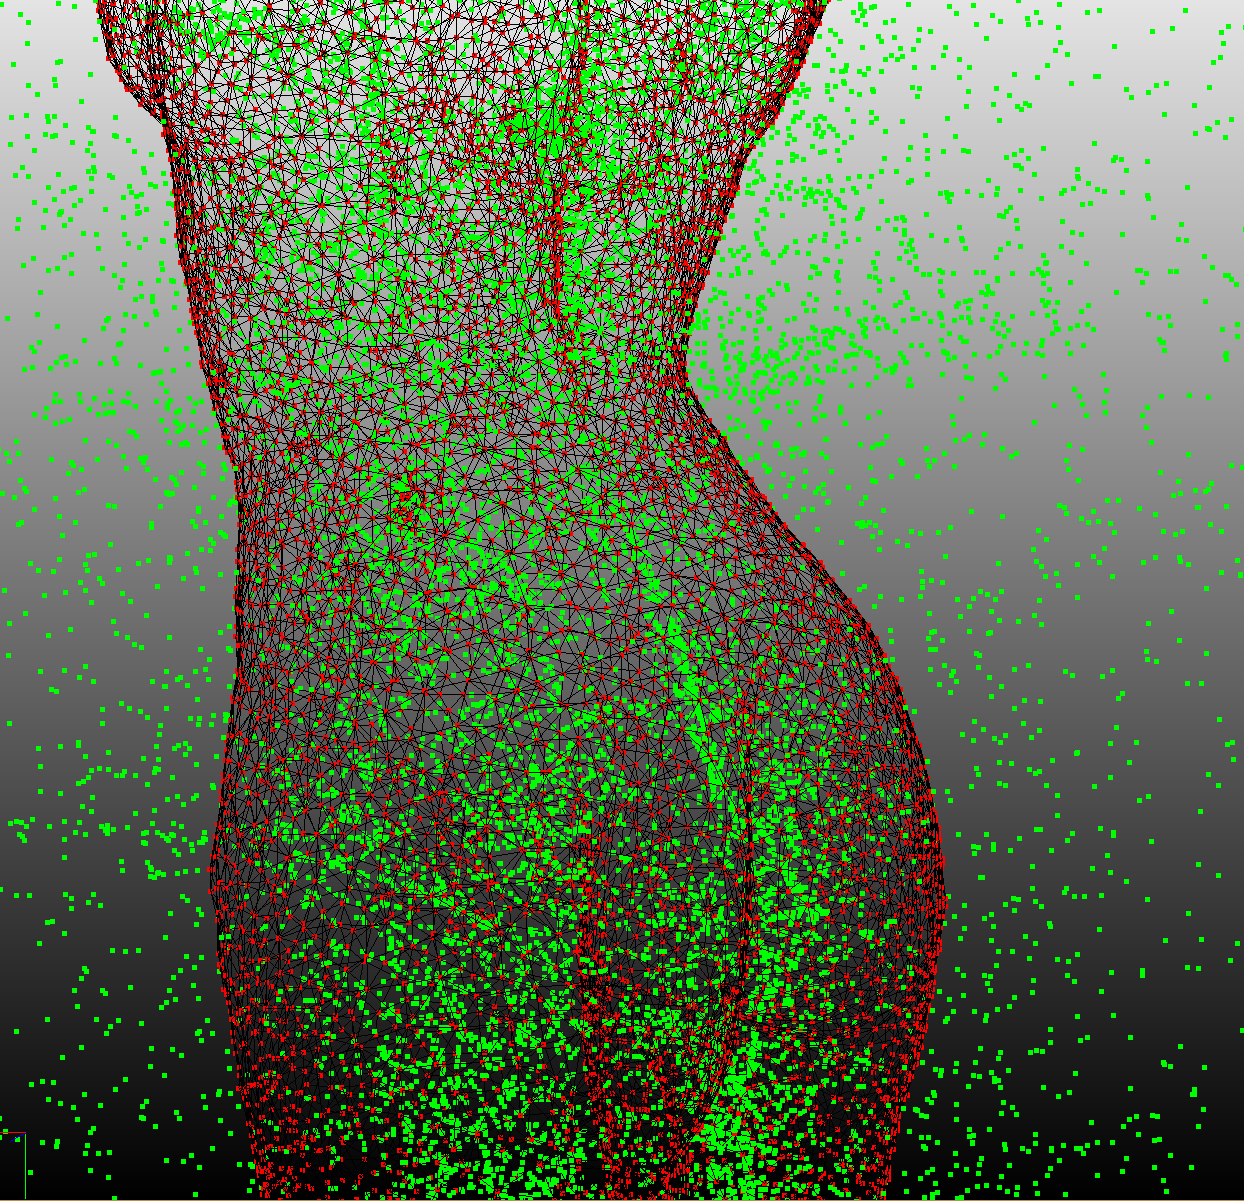
\includegraphics[width=0.32\textwidth]{img/woman02.png}
     \label{fig:woman2}
  }\hspace{-3mm}
  \subfigure[]{
    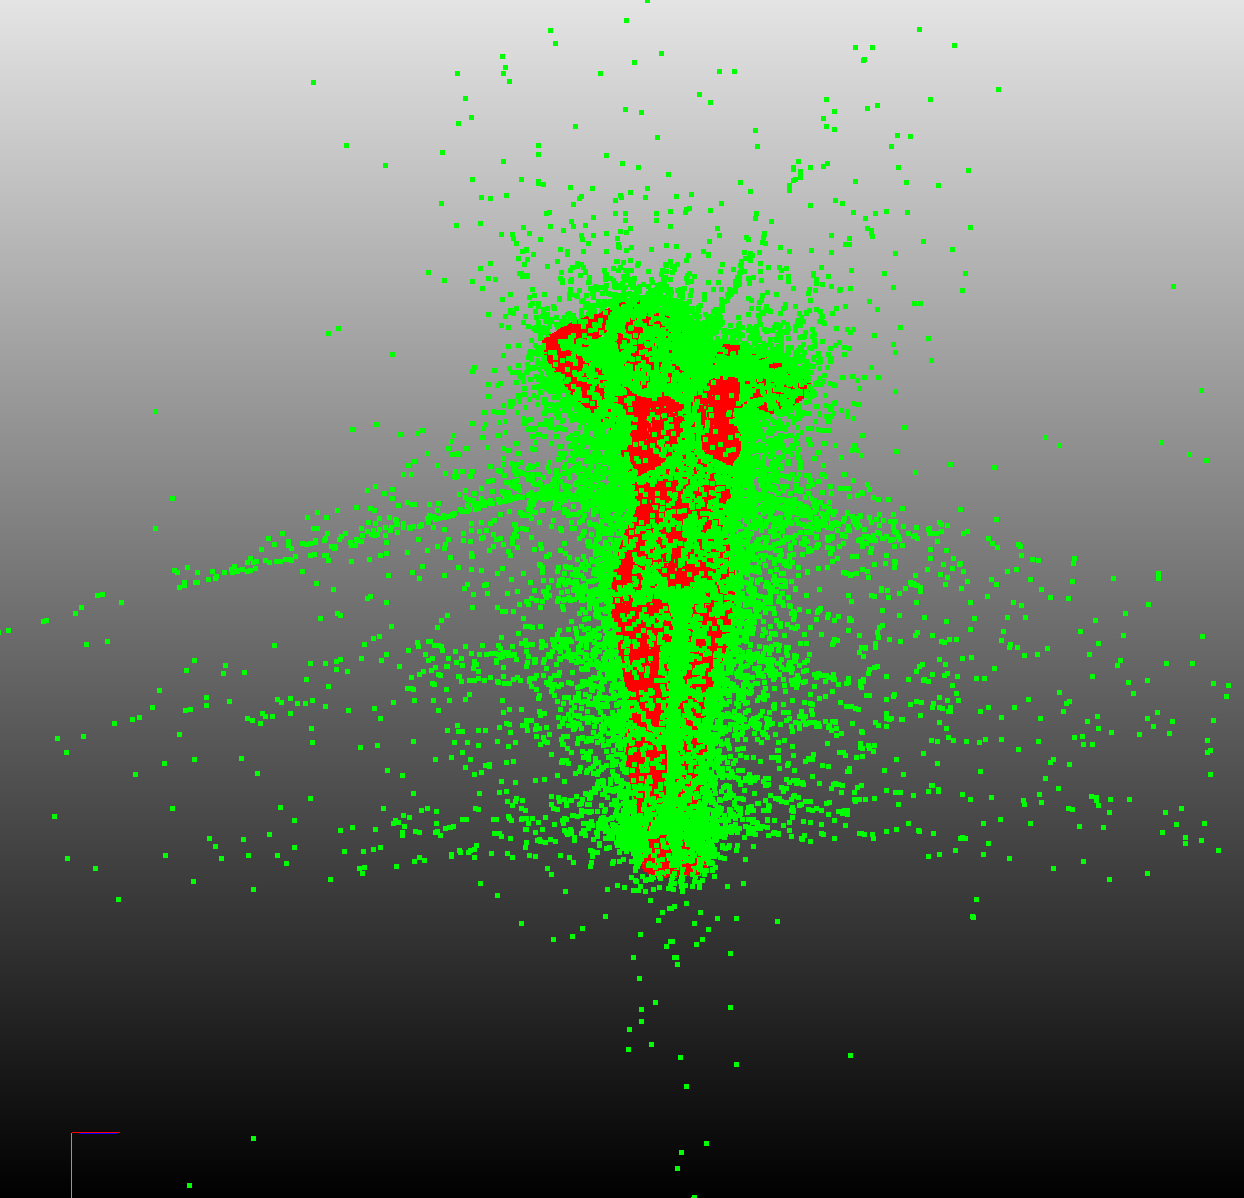
\includegraphics[width=0.32\textwidth]{img/woman03.png}
     \label{fig:woman3}
  }\hspace{-3mm}
  \caption{An woman example \label{fig:woman}}
\end{figure*}
\begin{figure*}[hbt]
 \centering
  \subfigure[]{
    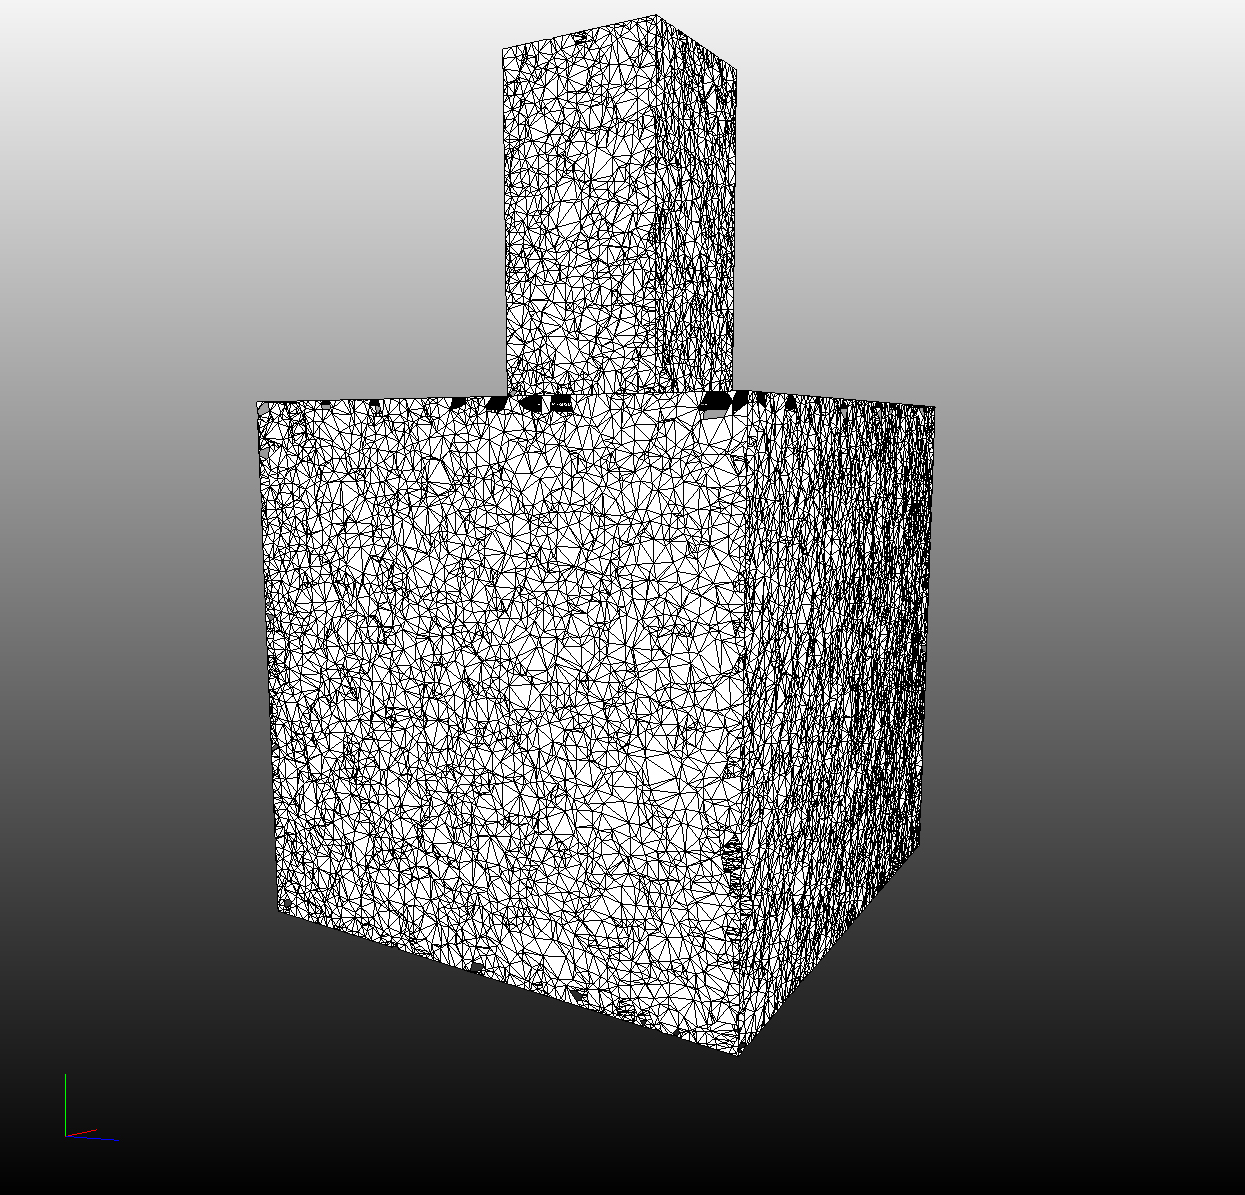
\includegraphics[width=0.32\textwidth]{img/T01.png}
    \label{fig:t1}
  }\hspace{-3mm}
  \subfigure[]{
     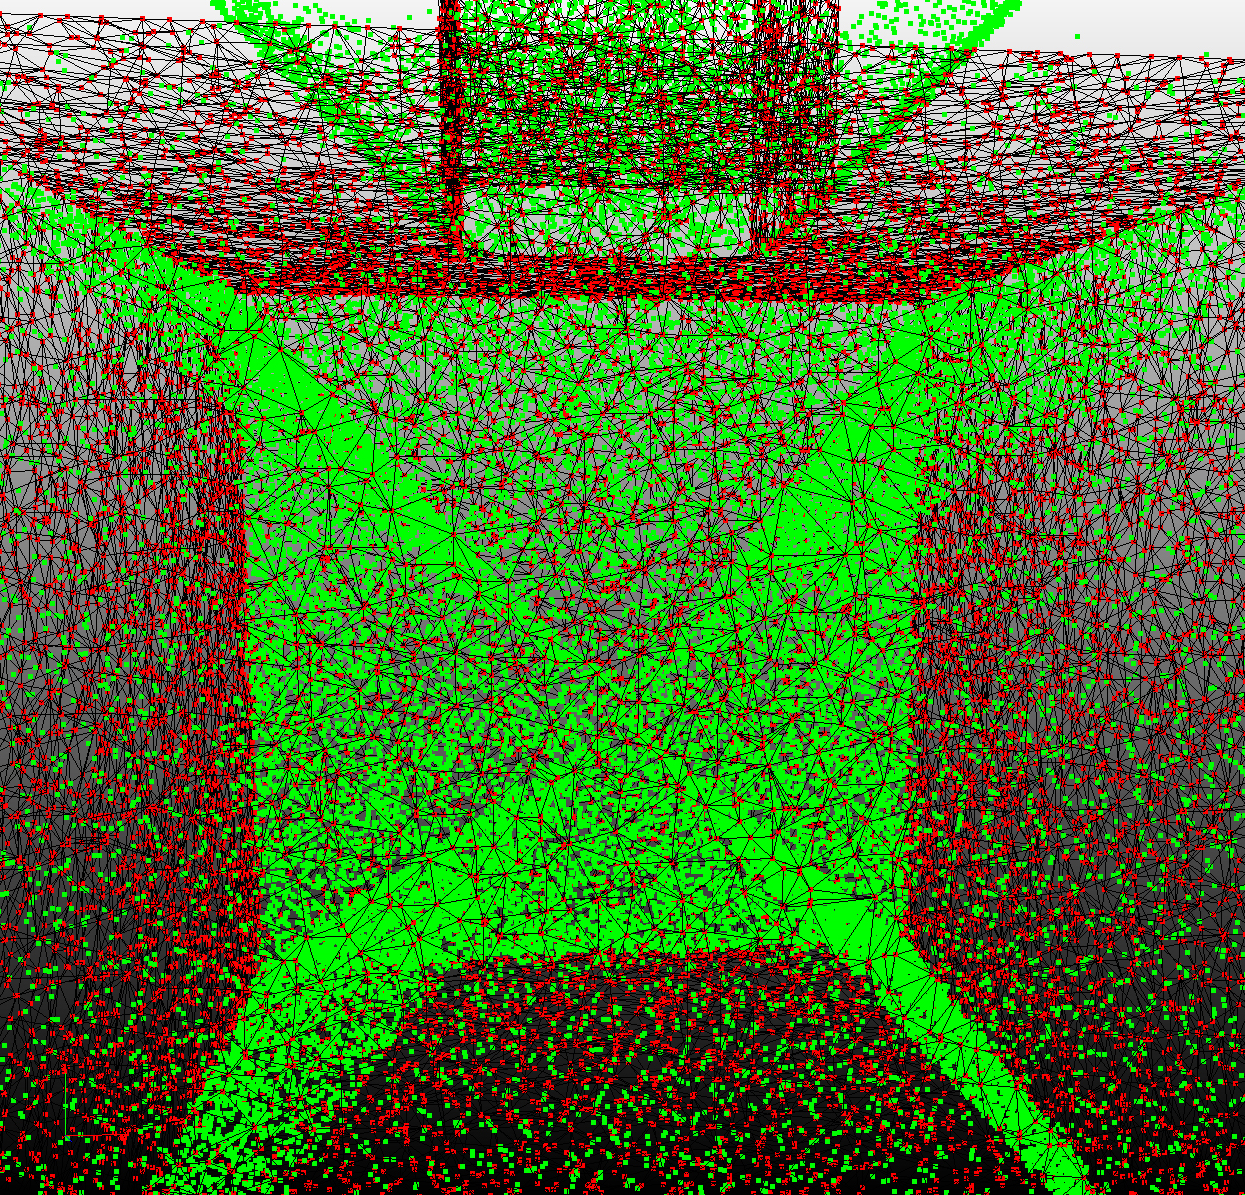
\includegraphics[width=0.32\textwidth]{img/T02.png}
     \label{fig:t2}
  }\hspace{-3mm}
  \subfigure[]{
    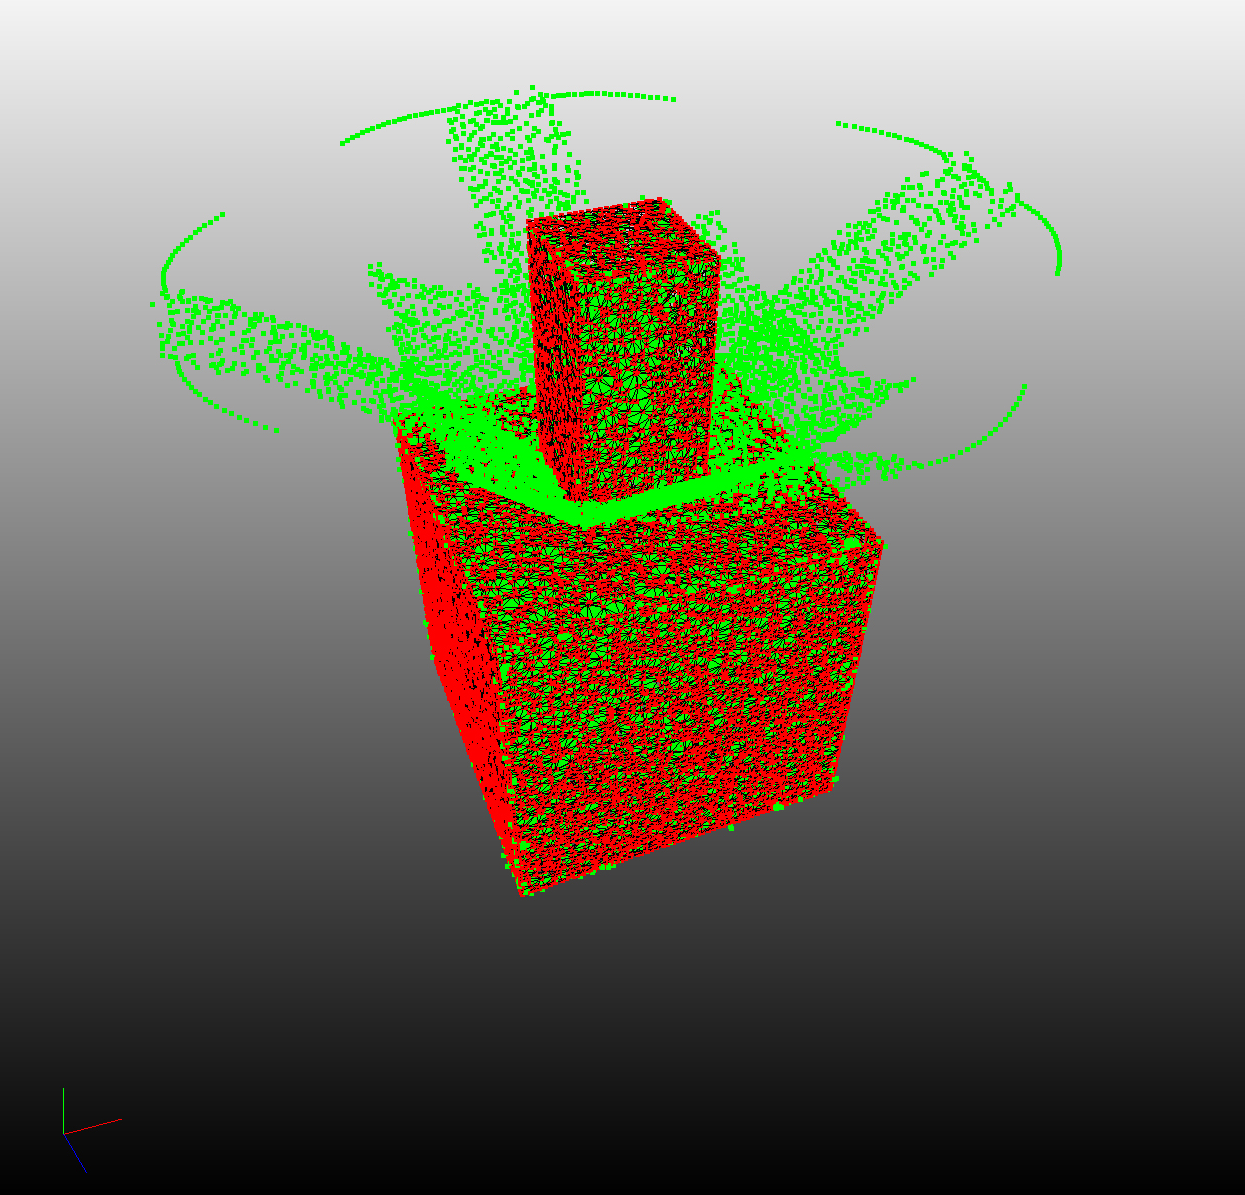
\includegraphics[width=0.32\textwidth]{img/T03.png}
     \label{fig:t3}
  }\hspace{-3mm}
  \caption{A 'T' example \label{fig:T}}
\end{figure*}
\begin{figure*}[hbt]
 \centering
  \subfigure[]{
    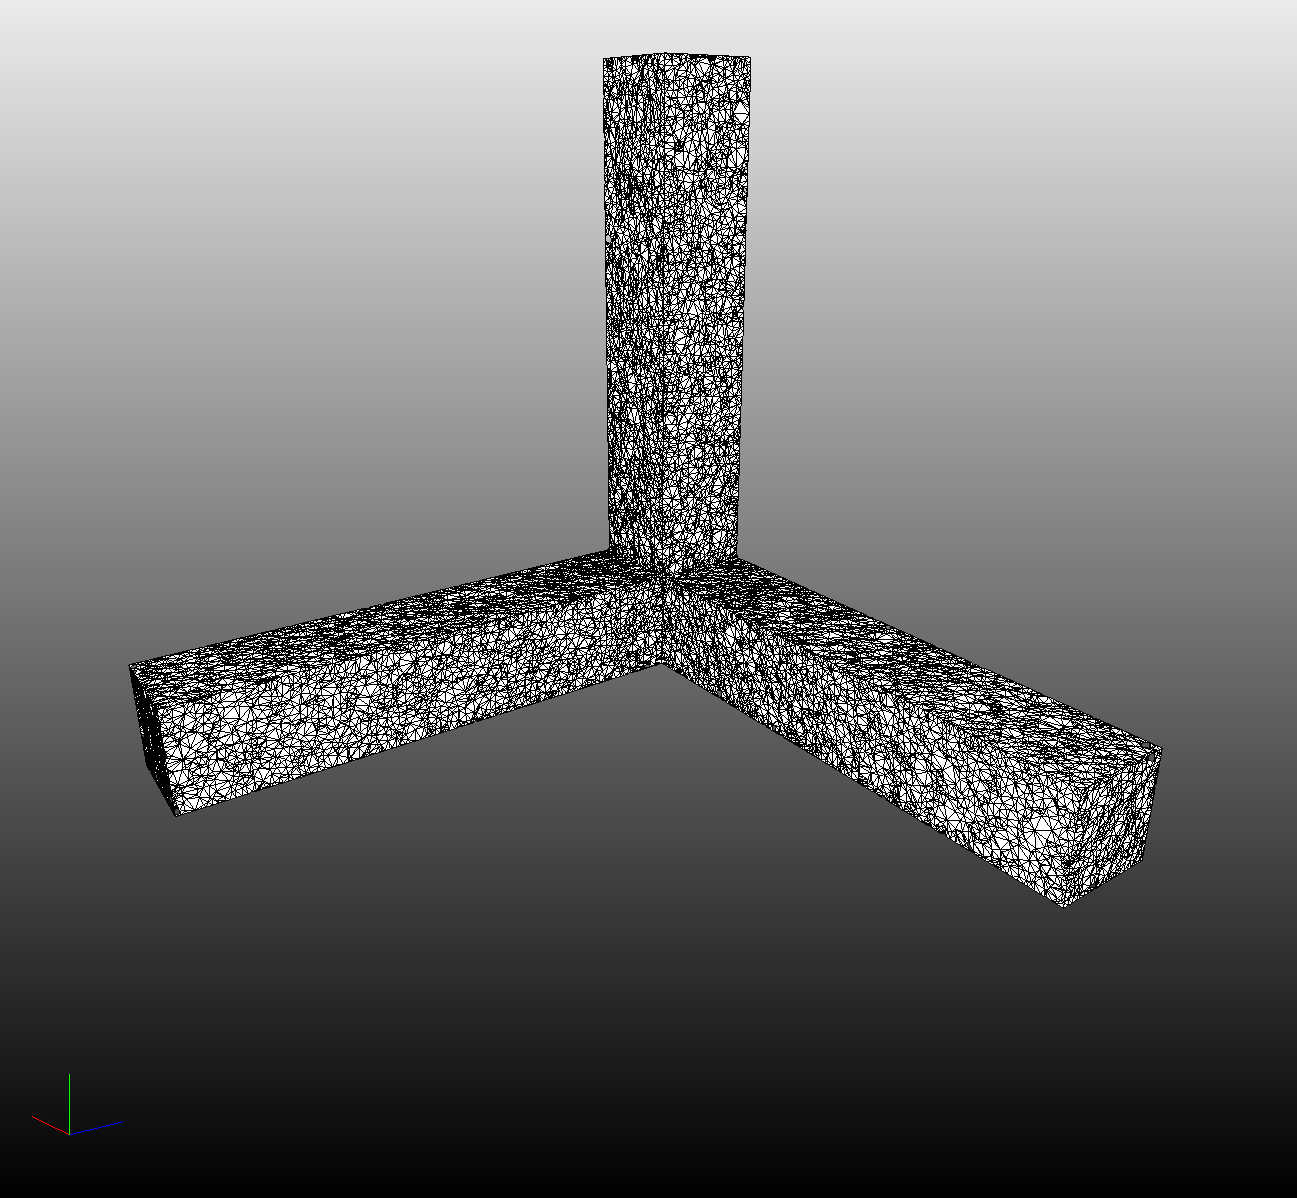
\includegraphics[width=0.32\textwidth]{img/Y01.png}
    \label{fig:y1}
  }\hspace{-3mm}
  \subfigure[]{
     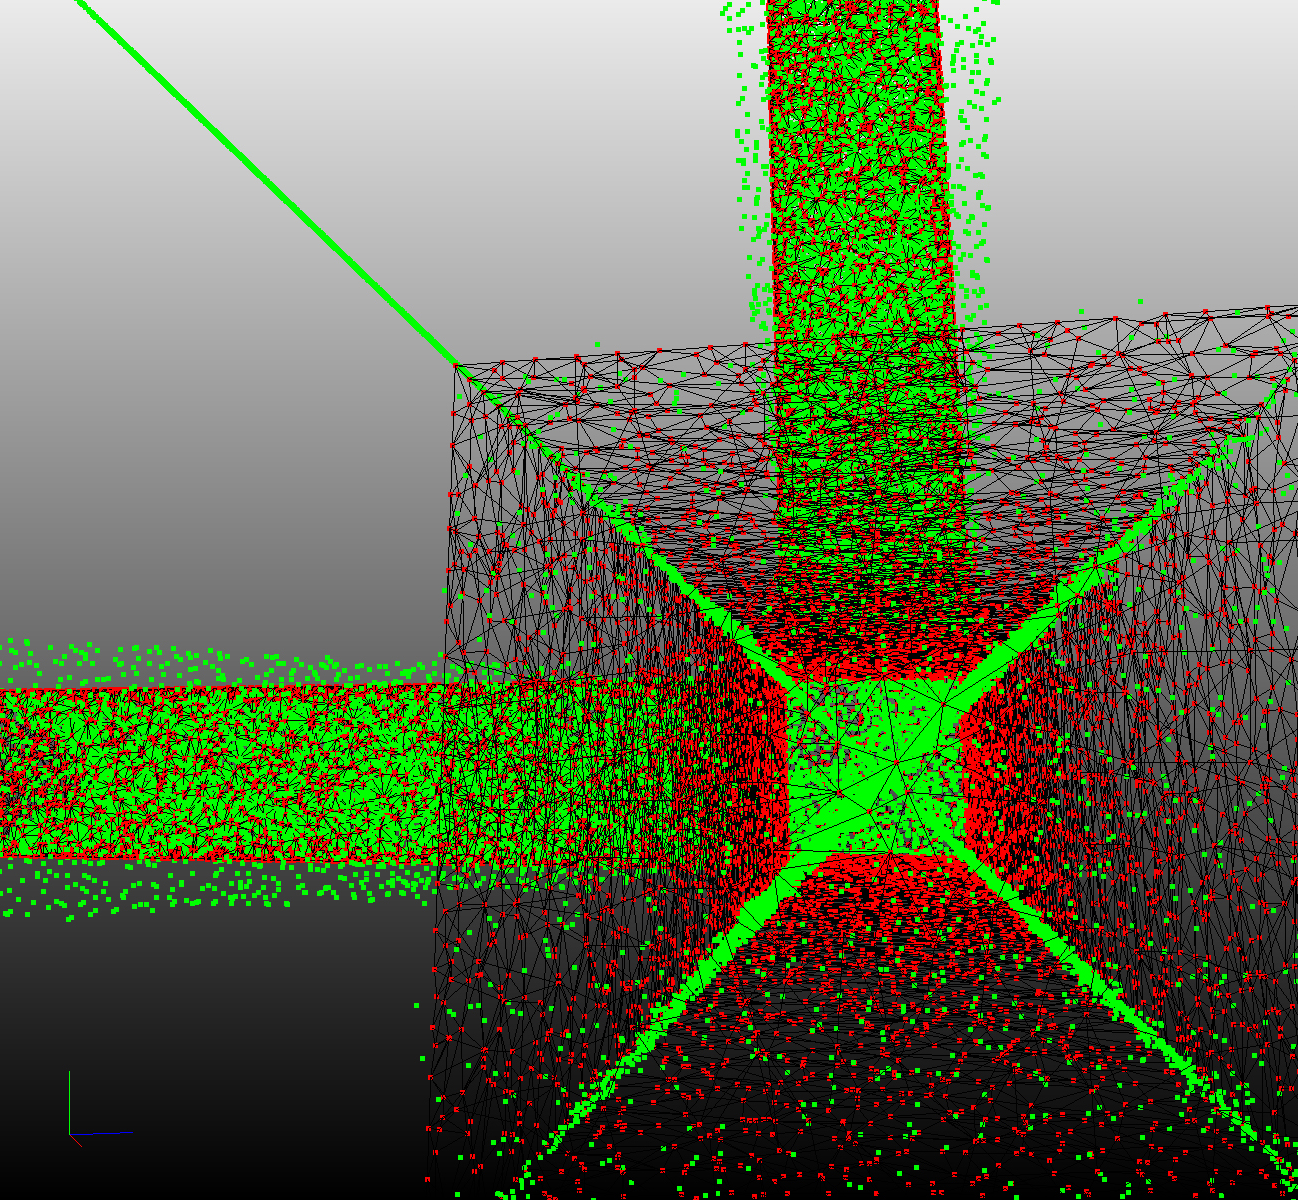
\includegraphics[width=0.32\textwidth]{img/Y02.png}
     \label{fig:y2}
  }\hspace{-3mm}
  \subfigure[]{
    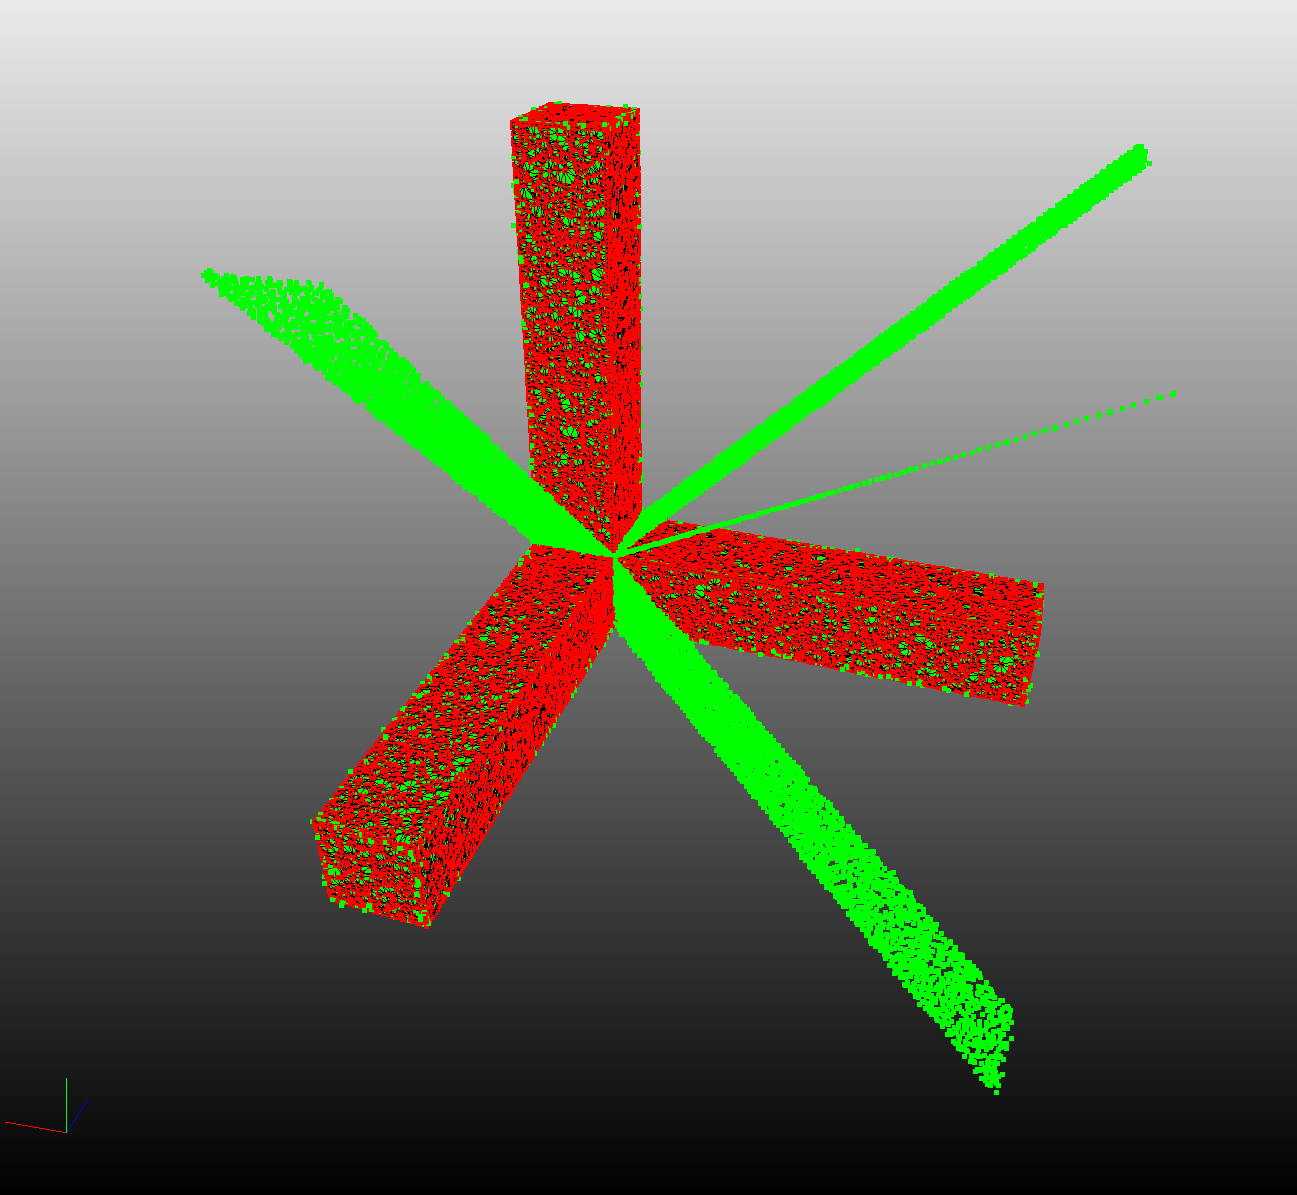
\includegraphics[width=0.32\textwidth]{img/Y03.png}
     \label{fig:y3}
  }\hspace{-3mm}
  \caption{An 'Y' example \label{fig:Y}}
\end{figure*}
\begin{figure*}[hbt]
 \centering
  \subfigure[]{
    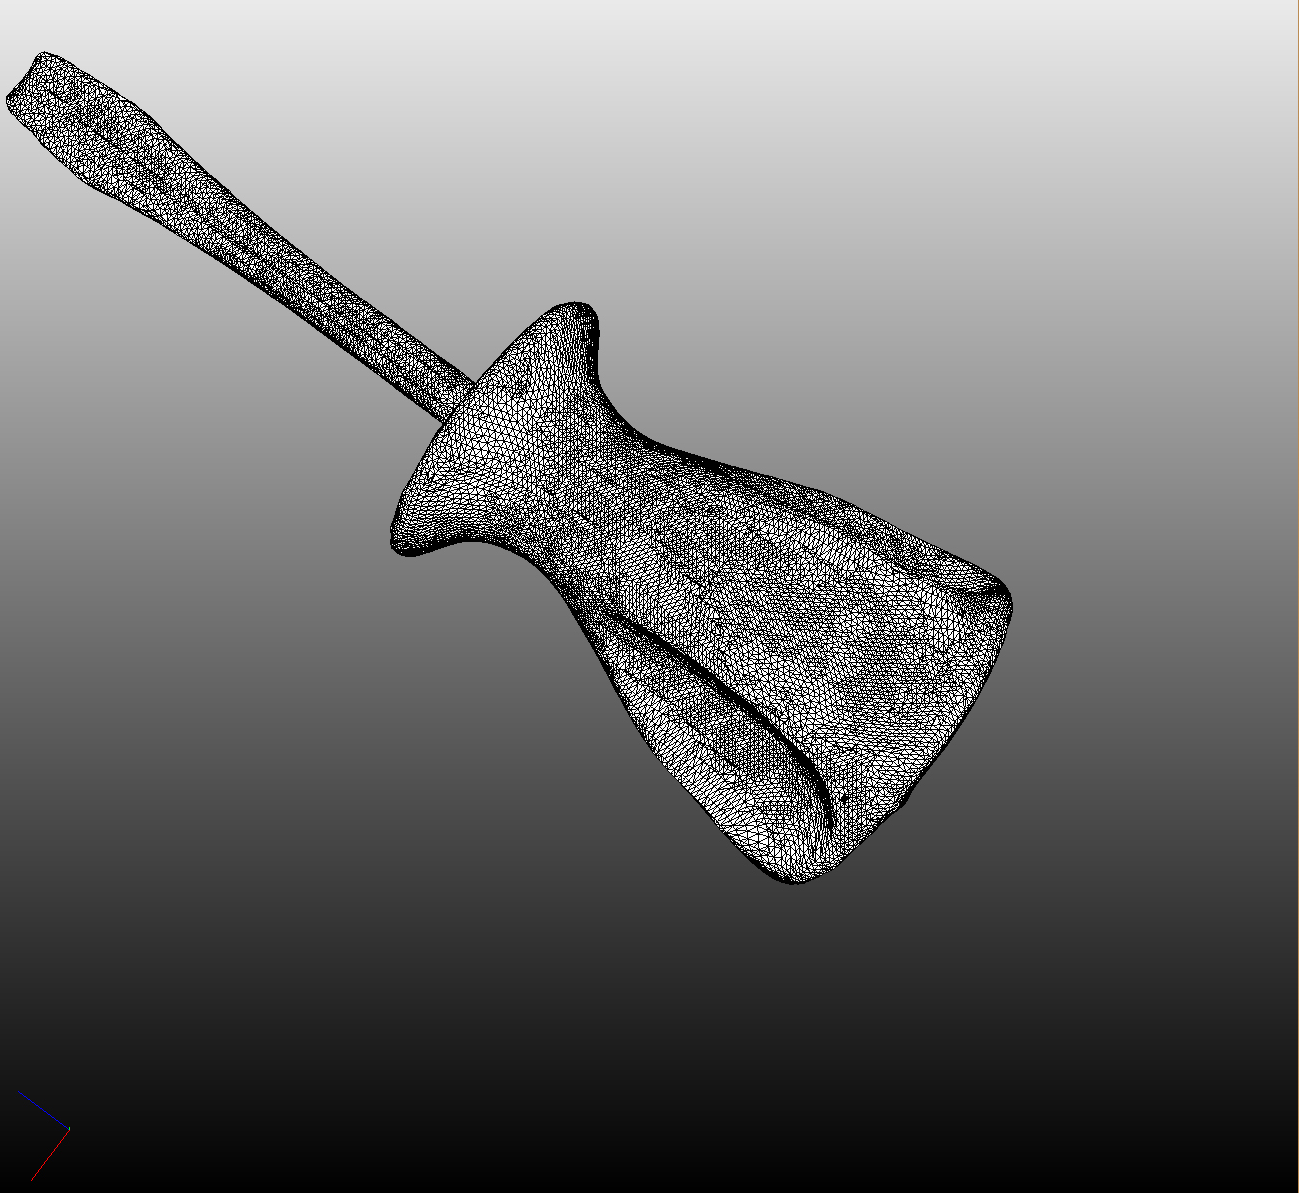
\includegraphics[width=0.32\textwidth]{img/sd01.png}
    \label{fig:sd13}
  }\hspace{-3mm}
  \subfigure[]{
     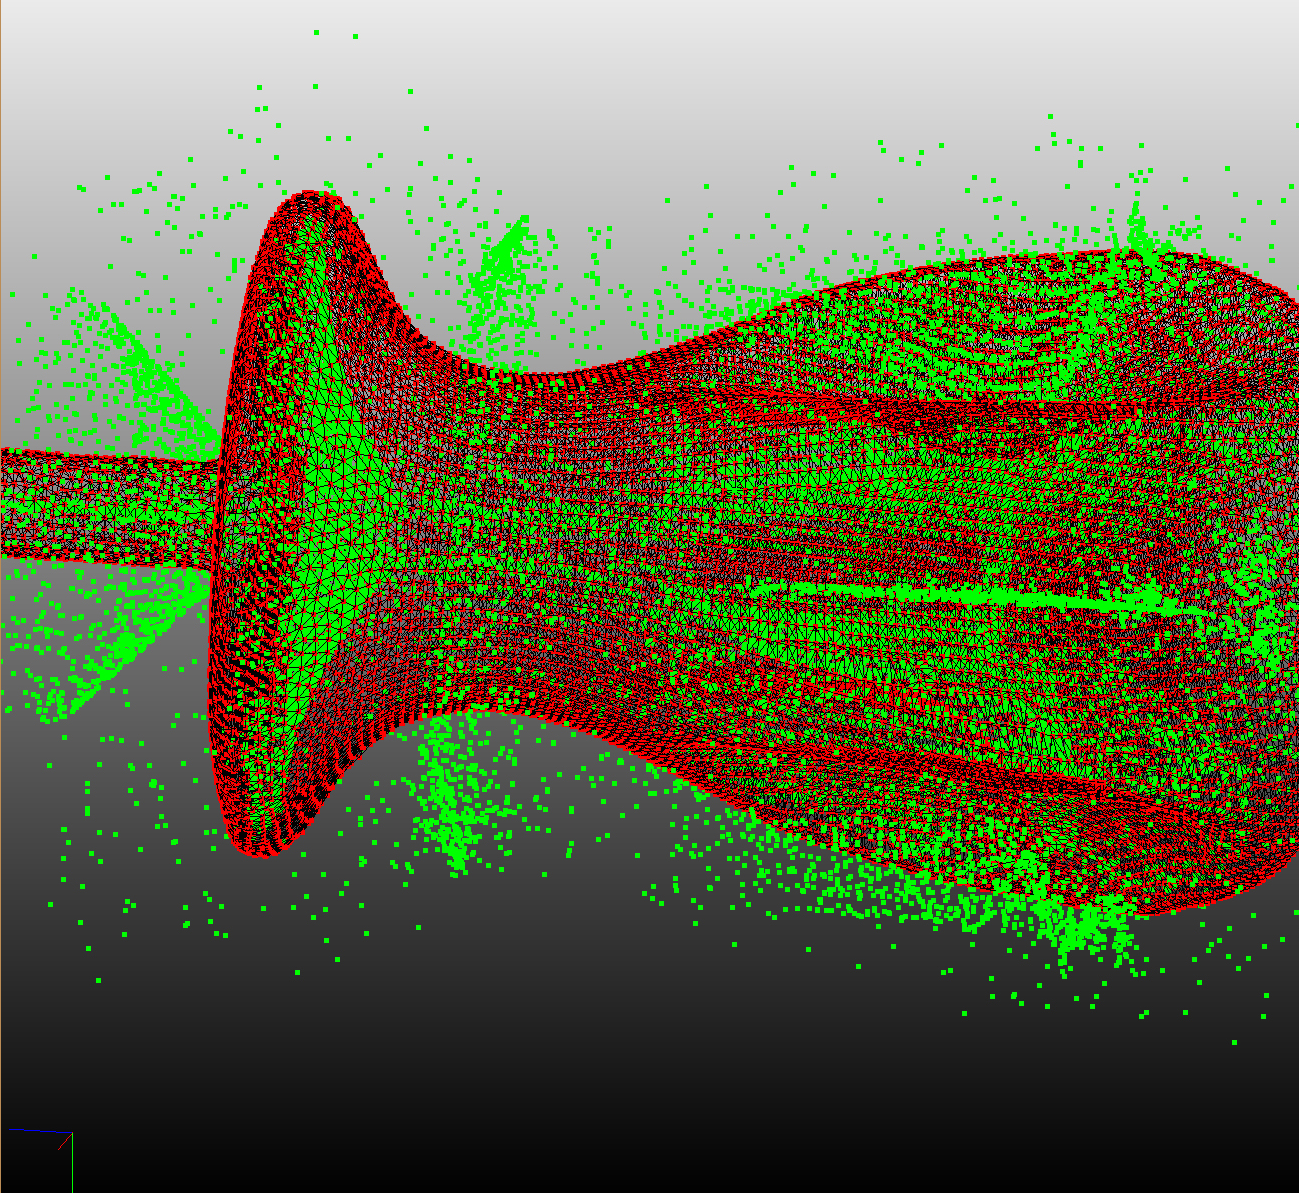
\includegraphics[width=0.32\textwidth]{img/sd02.png}
     \label{fig:sd2}
  }\hspace{-3mm}
  \subfigure[]{
    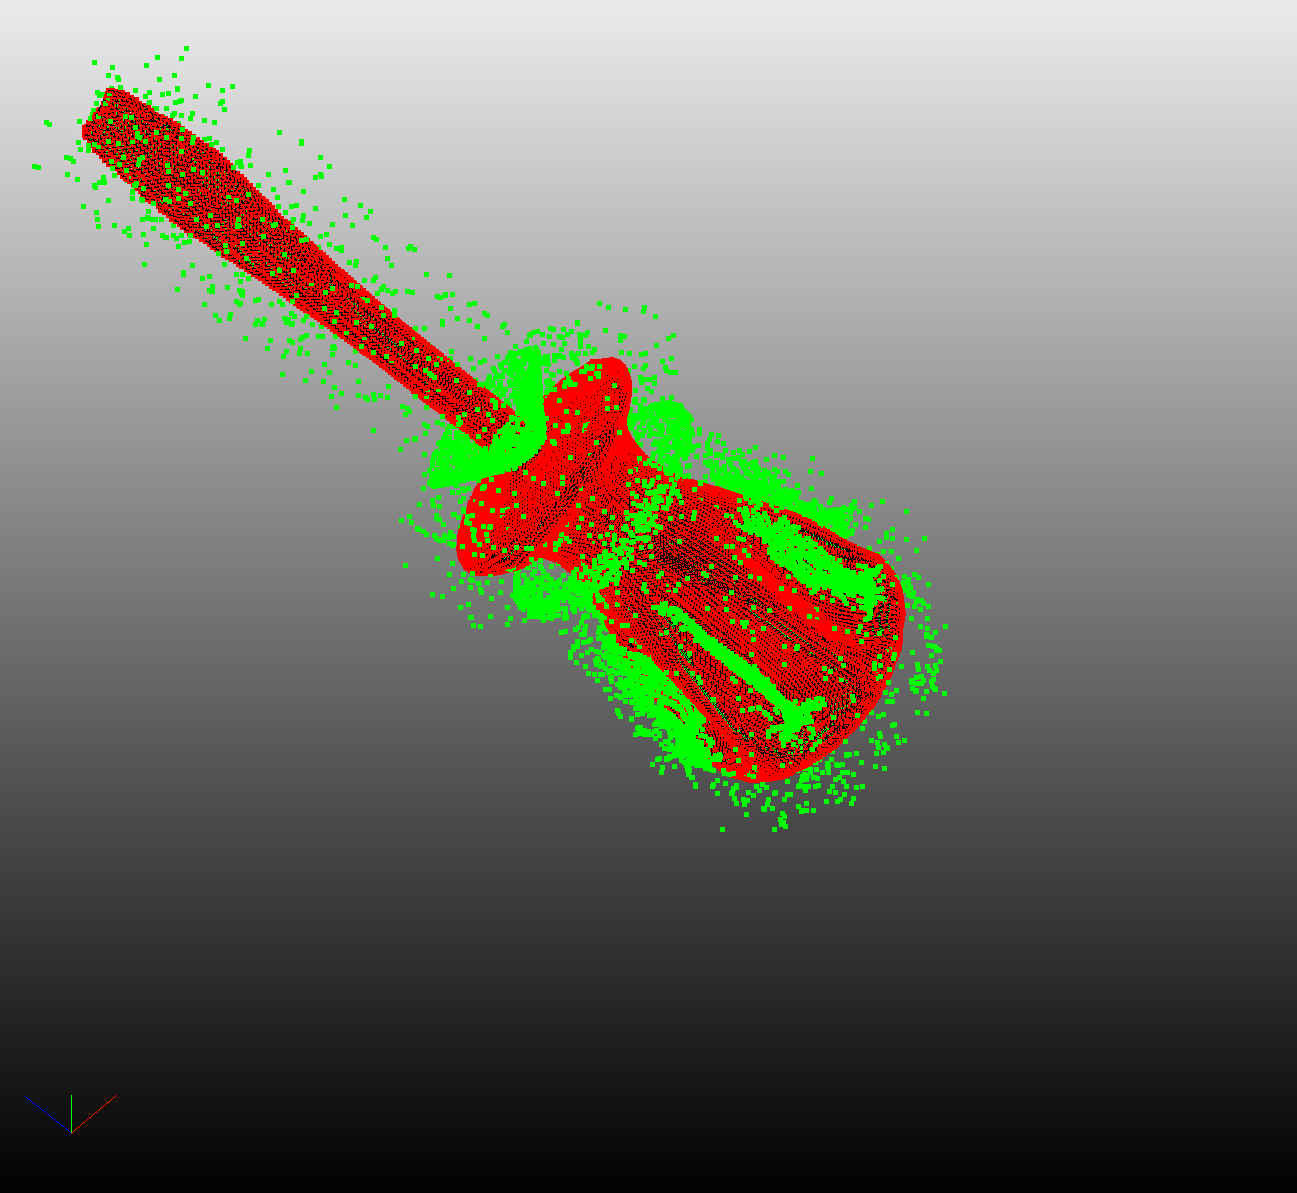
\includegraphics[width=0.32\textwidth]{img/sd03.png}
     \label{fig:sd3}
  }\hspace{-3mm}
  \caption{A screwdriver example \label{fig:sd}}
\end{figure*}
\begin{figure*}[hbt]
 \centering
  \subfigure[]{
    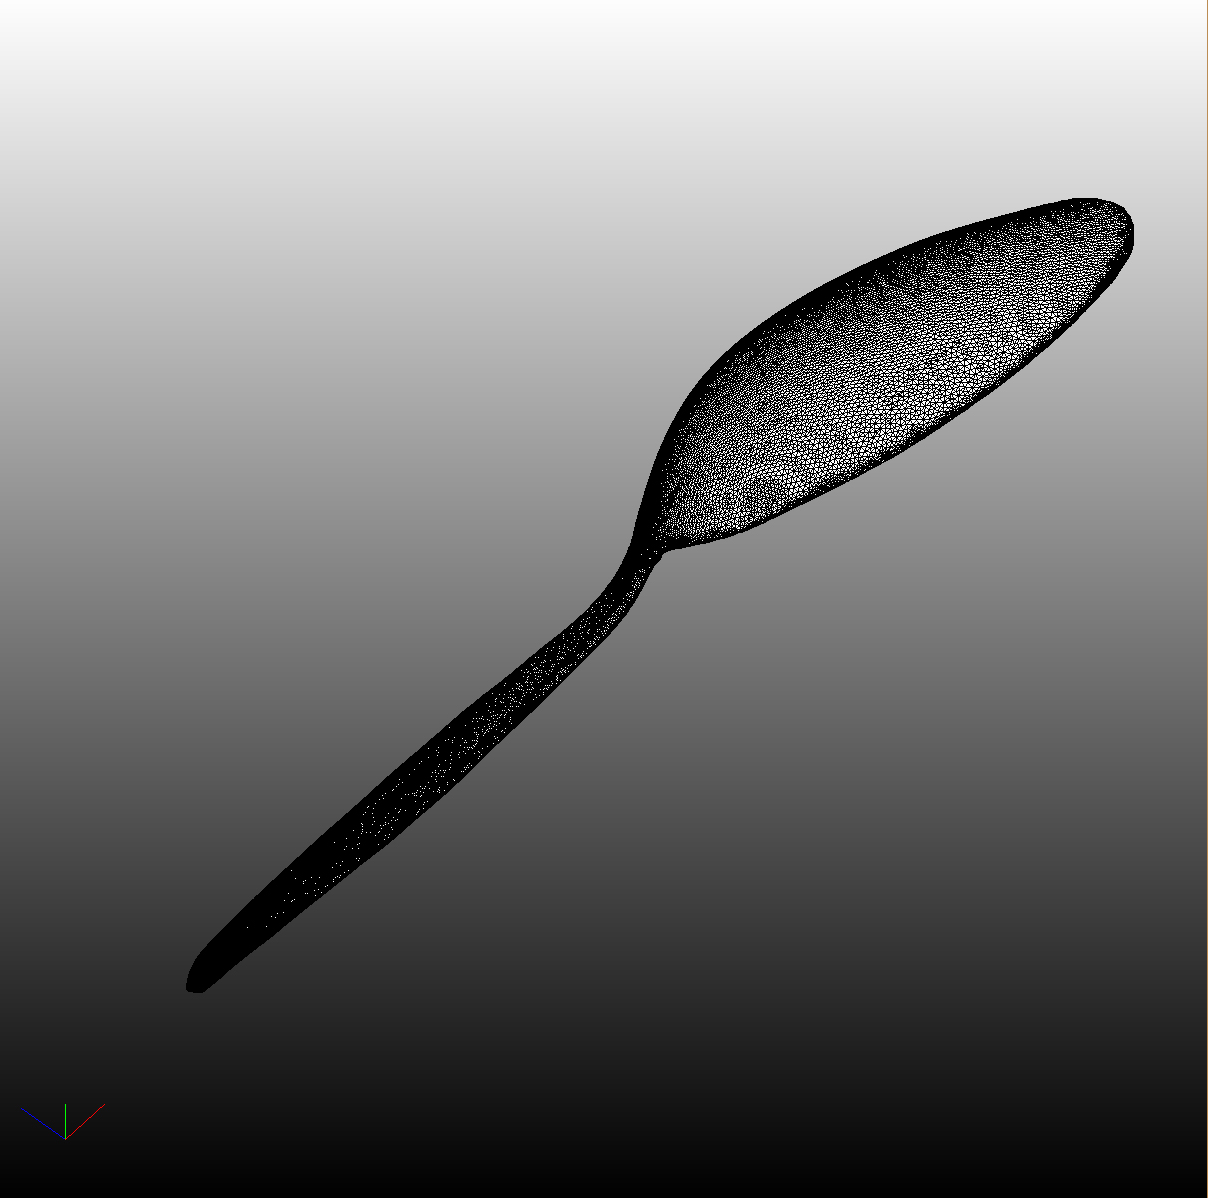
\includegraphics[width=0.32\textwidth]{img/spoon01.png}
    \label{fig:spoon1}
  }\hspace{-3mm}
  \subfigure[]{
     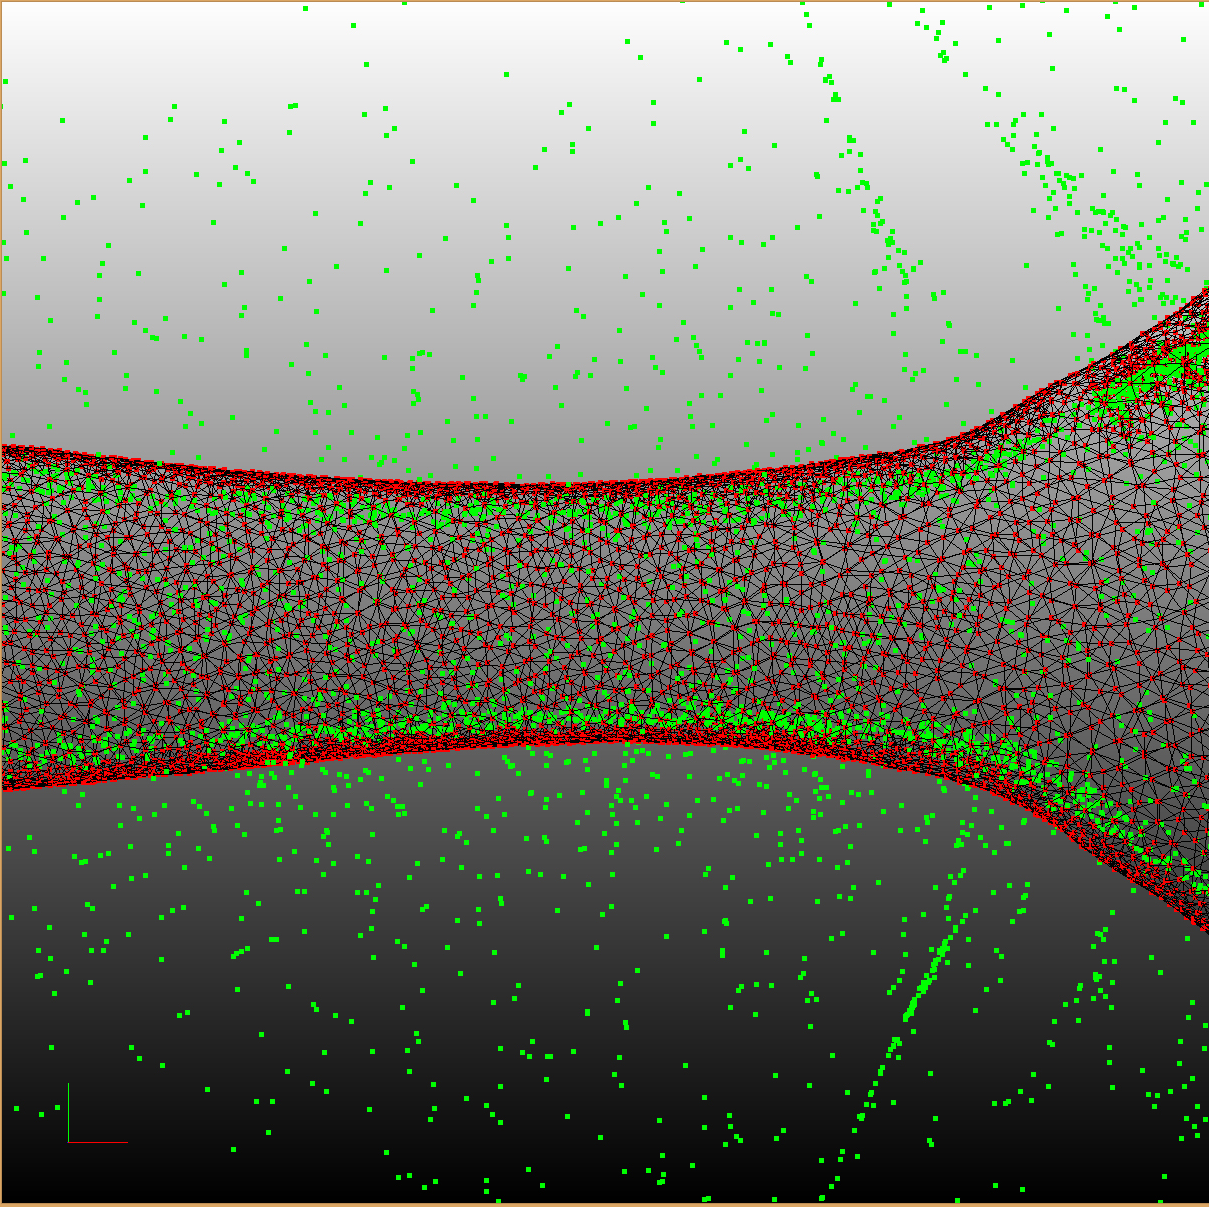
\includegraphics[width=0.32\textwidth]{img/spoon02.png}
     \label{fig:spoon2}
  }\hspace{-3mm}
  \subfigure[]{
    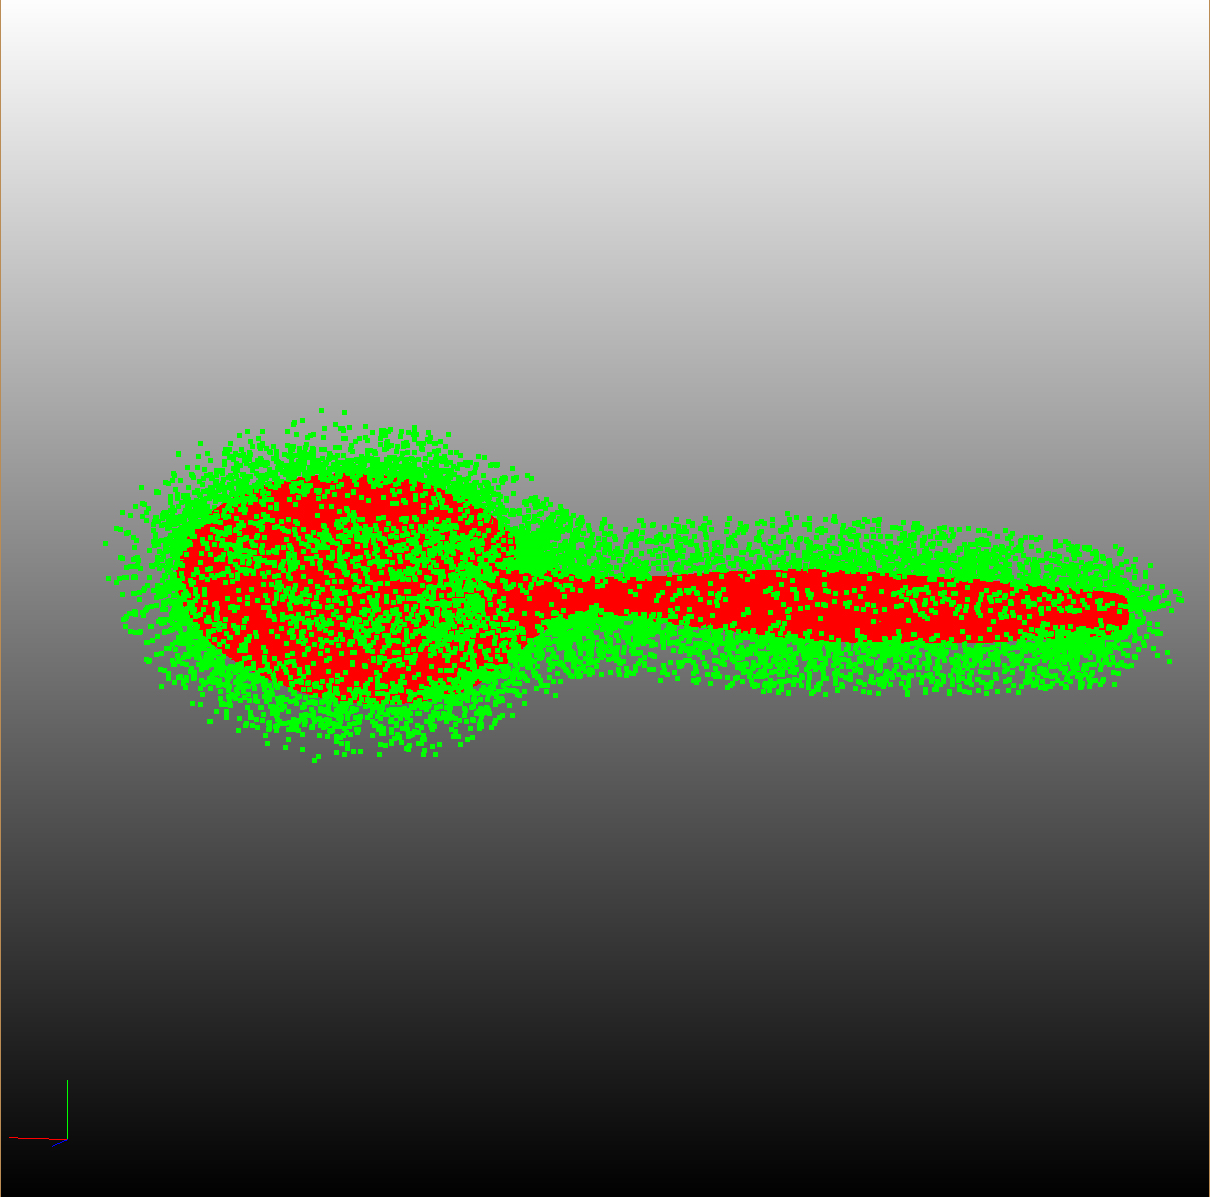
\includegraphics[width=0.32\textwidth]{img/spoon03.png}
     \label{fig:spoon3}
  }\hspace{-3mm}
  \caption{A spoon example \label{fig:spoon}}
\end{figure*}
\begin{figure*}[hbt]
 \centering
  \subfigure[]{
    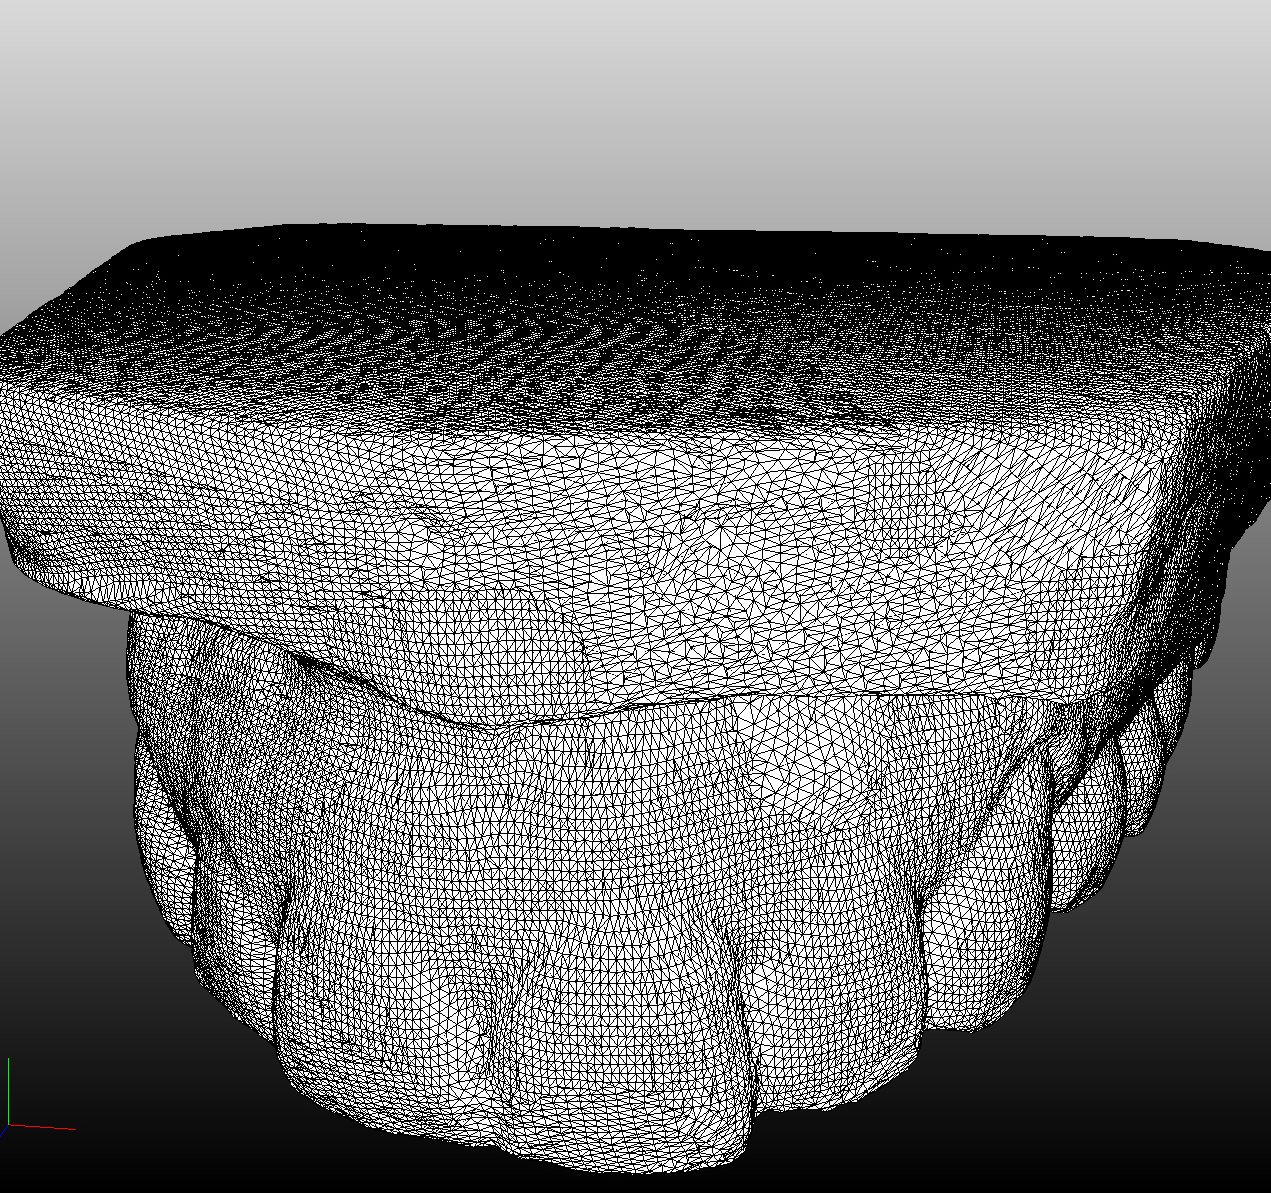
\includegraphics[width=0.32\textwidth]{img/teeth01.png}
    \label{fig:teeth1}
  }\hspace{-3mm}
  \subfigure[]{
     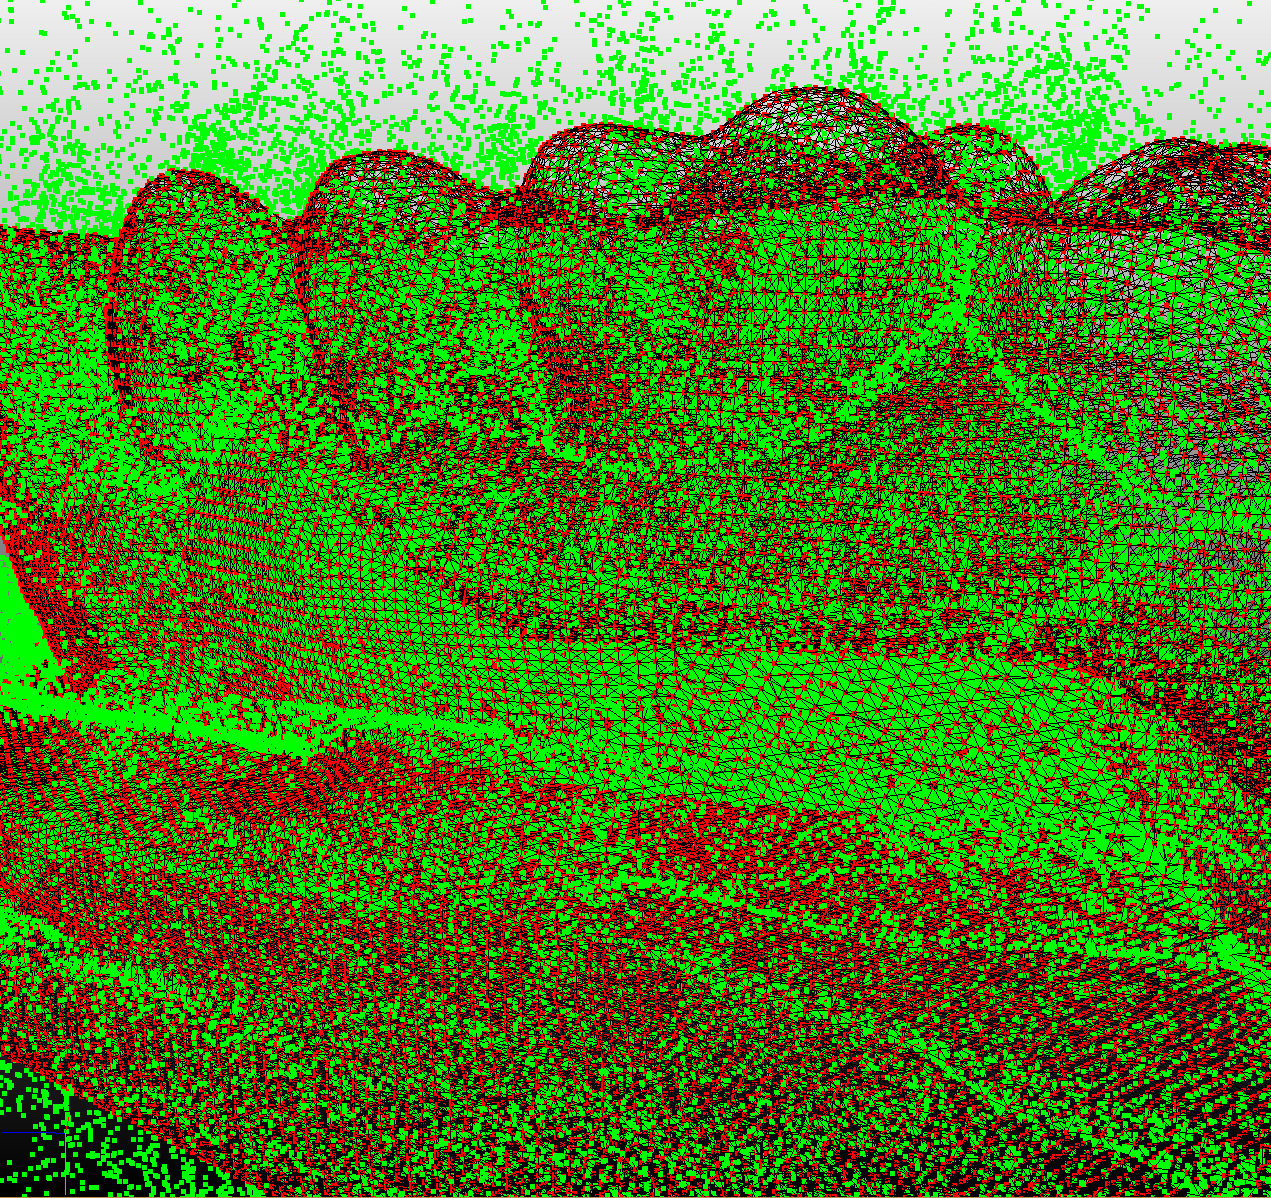
\includegraphics[width=0.32\textwidth]{img/teeth02.png}
     \label{fig:teeth2}
  }\hspace{-3mm}
  \subfigure[]{
    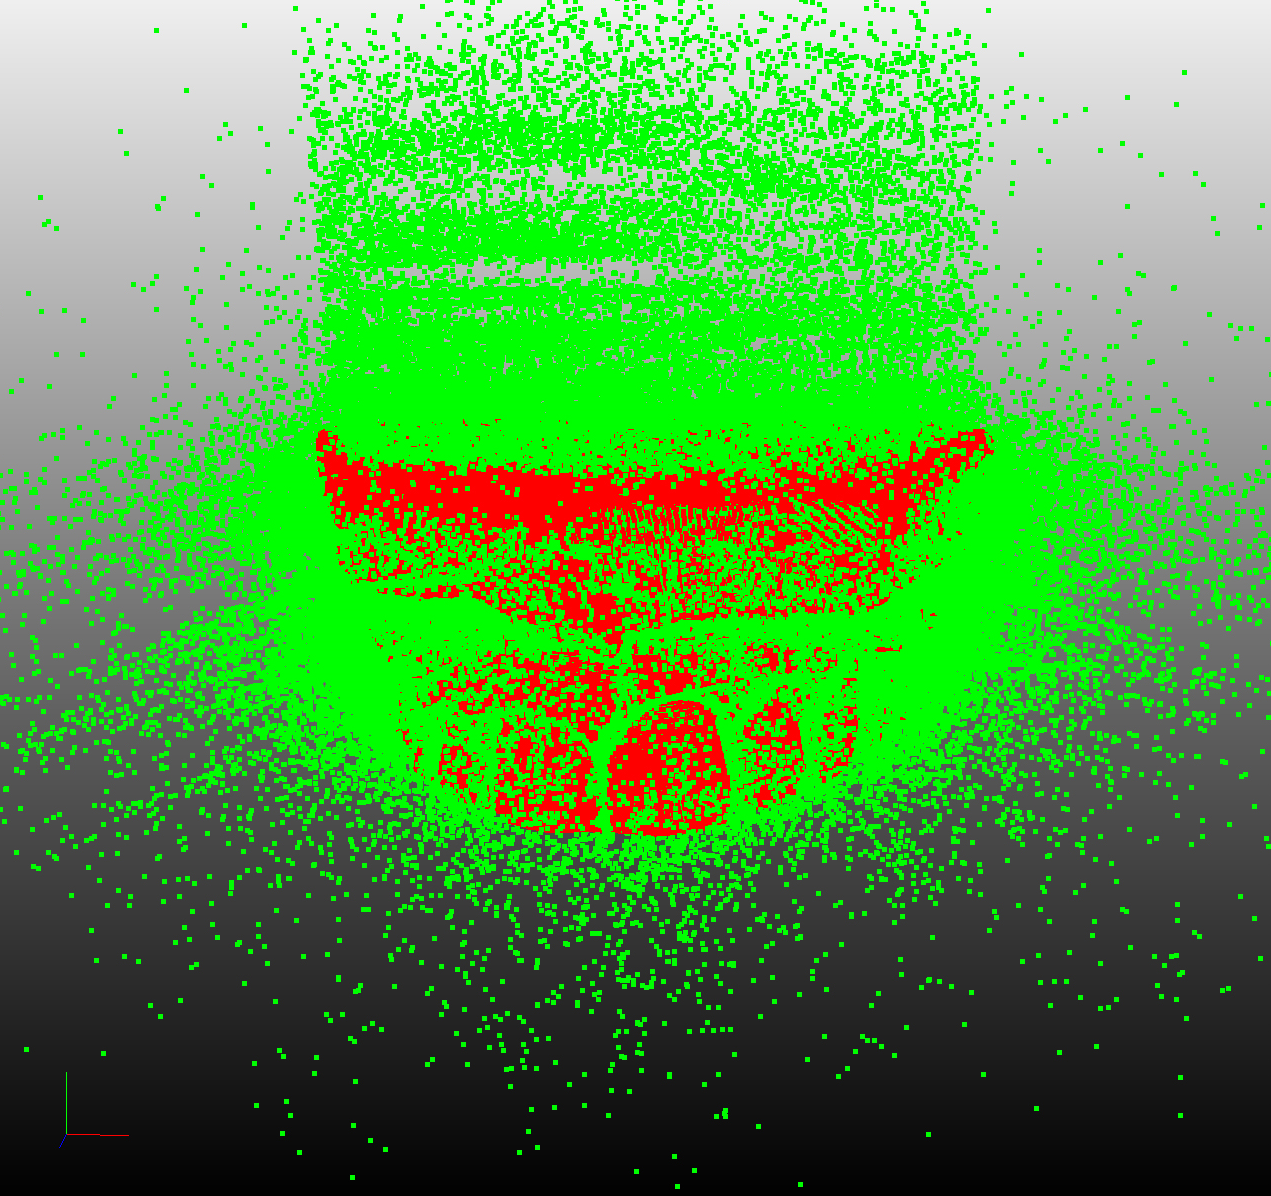
\includegraphics[width=0.32\textwidth]{img/teeth03.png}
     \label{fig:teeth3}
  }\hspace{-3mm}
  \caption{A teeth example \label{fig:teeth}}
\end{figure*}
\end{document}




